\documentclass[11pt,oneside]{book}

\usepackage[T1]{fontenc}
\usepackage[french]{babel}

\usepackage[utf8]{inputenc}
\usepackage{graphicx}
\usepackage{grffile}
\usepackage{longtable}
\usepackage{wrapfig}
\usepackage{rotating}
\usepackage[normalem]{ulem}
\usepackage{amsmath}
\usepackage{textcomp}
\usepackage{amssymb}
\usepackage{capt-of}
\usepackage[colorlinks=true,linkcolor=black,citecolor=black]{hyperref}
\usepackage{textgreek}
\usepackage{minted}
\usepackage{framed}
\usepackage{mdframed}
\usepackage{geometry}
\usepackage{titlesec}
\usepackage{pdfpages}
\usepackage{fancyhdr}
\usepackage{colortbl}
\usepackage[dvipsnames]{xcolor}
\usepackage[textwidth=16mm]{todonotes}
\usepackage{color}

\newcommand{\as}[1]{\todo[color=green!40,size=\tiny,caption={}]{#1}}
\newcommand{\asi}[1]{\todo[inline,caption={},color=green!40]{#1}}

\newcommand{\hlink}[2]{\hyperlink{#1}{\color{magenta} #2}}

\geometry{
a4paper,
left=18mm,
right=18mm,
top=20mm,
bottom=20mm
}

\begin{document}


\includepdf[pages=-]{page1.pdf}

\pagestyle{empty}
\fontfamily{cmss}
\selectfont

\setlength{\parindent}{4mm}

\setcounter{tocdepth}{1}
\tableofcontents
\pagenumbering{gobble}

\chapter{Introduction}
\pagenumbering{arabic}
\setcounter{page}{1}
\pagestyle{fancy}
\fancyhf{}
\cfoot[\thepage]{\thepage}

Ce projet nous a été proposé par l’équipe \href{https://www-intuidoc.irisa.fr/}{IntuiDoc} de l’\href{https://www.irisa.fr/}{IRISA}, en étroite collaboration avec la startup \href{http://www.doptim.eu}{Doptim} et avec le soutien de Jean-Yves LE CLERC, conservateur du patrimoine aux \href{http://archives.ille-et-vilaine.fr/fr}{archives départementales} d'Ille-et-Vilaine. Tout au long de l’année, nous serons encadrés par Bertrand COÜASNON, enseignant-chercheur membre d'IntuiDoc, Erwan FOUCHÉ, chef de projet chez \href{https://www.soprasteria.com/fr}{Sopra Steria}, Julien BOUVET, ingénieur chez Sopra Steria également. Nous serons aussi accompagnés par Sophie TARDIVEL, responsable et \textit{data scientist} chez Doptim.

\paragraph{}
Dans ce rapport, nous rappellerons le contexte du projet qui justifie certains choix de conception. Nous décrirons ensuite l’architecture logicielle générale de notre projet ainsi que les diagrammes de séquences illustrant le fonctionnement interne de ce dernier. Puis, nous décrirons plus en détail les deux itérations prévues, la première répondant simplement au cahier des charges, la seconde complétant l'ensemble des fonctionnalités décrites dans le rapport de spécification, et donnant plus d'importance à l'ergonomie de la solution logicielle.

% ---

\chapter{Contexte}

Ce projet a pour but de fournir un programme permettant de concevoir des bases d'apprentissage automatiquement pour l'entraînement de systèmes de reconnaissance d'écriture manuscrite. 
\chapter{Client}

\section{Choix du framework}

\paragraph{}
Pour réaliser l’interface Web de notre application, nous avons opté pour les technologies \texttt{HTML}, \texttt{CSS} et \href{https://angular.io/}{\texttt{Angular}}.

\paragraph{}
\texttt{HTML} nous permettra de réaliser le corps des pages de l’interface, à l’aide de balises définissant les différents éléments de la page pour structurer logiquement le contenu et y inclure des fichiers multimédias, comme des images, par exemple.

\paragraph{}
Avec le \texttt{CSS}, nous définirons la mise en forme et l’aspect graphique des pages \texttt{HTML}, soit l’agencement des éléments, leurs couleurs, leurs tailles et les polices de caractère.

\paragraph{}
Quant à \texttt{Angular}, il nous servira à gérer l’aspect dynamique de l’application web, comme la navigation d’une page de l’interface à une autre ou le passage de paramètres entre pages. \texttt{Angular} est un framework web développé en \texttt{TypeScript}, ce qui en fait l’un des plus utilisés pour le développement \textit{front-end} des applications web. Les principaux avantages d’\texttt{Angular} sont qu’il est mis à jour très régulièrement par les développeurs de Google, qu’il dispose d’une très bonne documentation et que le développement en \texttt{TypeScript} est stable, rapide et facile.

\paragraph{}
Ce sont des technologies largement utilisées par les développeurs et relativement simples d’utilisation. En outre, nous avons déjà été amenés à les utiliser dans des projets précédents, nous partons donc avec des bases. Nous avons fait le choix de la simplicité et de l’utilisation de technologies que nous avons déjà abordées afin de faciliter et d’accélérer la réalisation de l’interface, pour être en mesure de proposer un prototype fonctionnel pour la première itération le 27 février.

%-------------------------------------------------------------------------------
\section{Les différents composants de l'interface}

\paragraph{Première itération}
Pour la première itération, l’interface est réduite à sa forme la plus simple qui répond au cahier des charges, à savoir ouvrir un document de travail et valider ou invalider les transcriptions. L’IHM aura donc deux composants : la page d’accueil et la page de validation des annotations.

\paragraph{}
La page d’accueil permet à l’utilisateur de choisir le projet sur lequel il veut travailler ainsi que d'en créer de nouveaux en choisissant les documents qui le composent. Un projet possède plusieurs documents qui possèdent eux-mêmes plusieurs pages contenant les imagettes (\textit{PEA\_GEN\_6}). Cette page possède une liste des projets qui ont été ouverts auparavant dans l’application, ainsi qu’un bouton pour en créer un nouveau. Un clic sur ce bouton ouvre une nouvelle fenêtre pour que l’utilisateur parcoure ses documents et fasse son choix (spécifications \textit{PEA\_GEN\_7} et \textit{PEA\_GEN\_8}).

\newpage{}
\begin{mdframed}[frametitle={Figure 1 : Maquette de la page d'accueil de l'IHM}, innerbottommargin=10]
\begin{center}
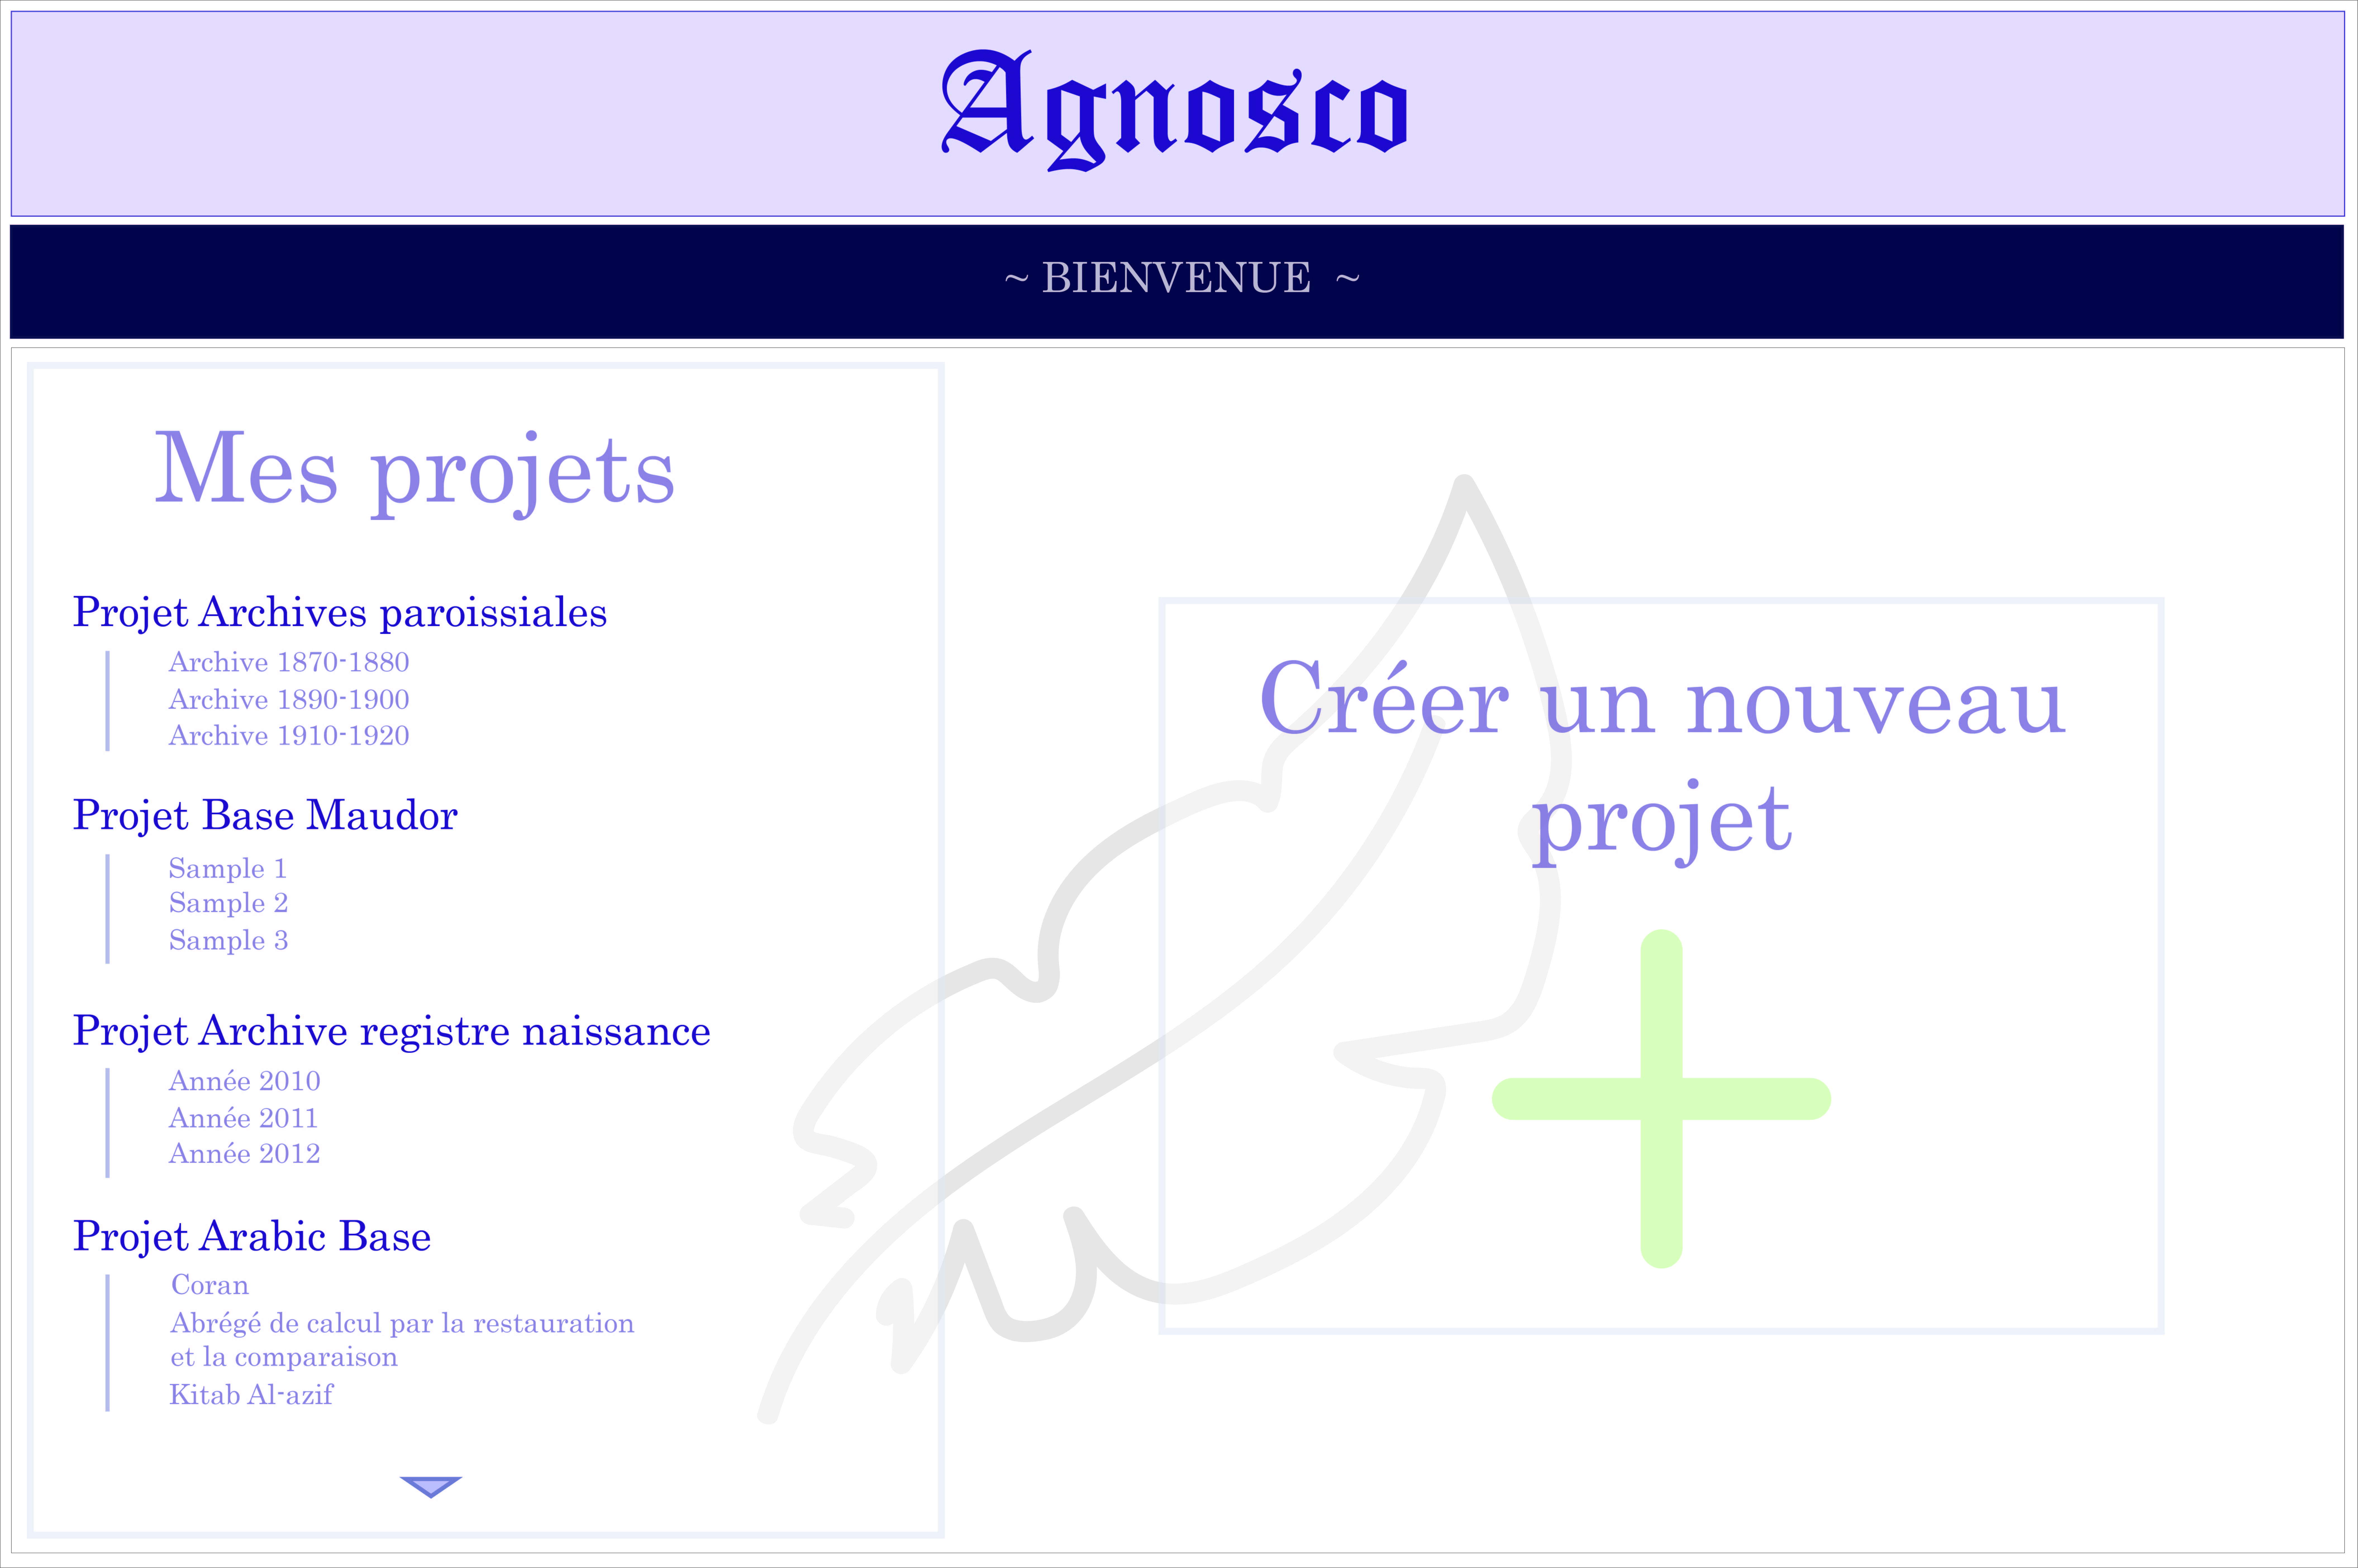
\includegraphics[scale=0.04]{assets/maquetteIHMaccueil.jpg}
\end{center}
\end{mdframed}

\paragraph{}
La page de validation (spécifications \textit{PVAL\_1} à \textit{PVAL\_7}), comme son nom l’indique, permet de valider ou d’invalider les transcriptions de la base de données relatives au document ouvert (\textit{PEA\_GEN\_1}). Ces transcriptions ayant été réalisées par des humains, elles sont considérées comme vraies et l’utilisateur pourrait les invalider seulement s’il manque des mots ou si l’imagette est jugée peu pertinente pour l’apprentissage (par exemple, si le texte est presque illisible ou si l’imagette ne contient pas de texte du tout).
\newline{}
Pour ce faire, les imagettes sont affichées les unes à la suite des autres et chacune possède sa transcription située dans une zone de texte en dessous. Les imagettes sont affichées par groupe de cinq ou six. Une croix à côté de chaque imagette permet à l’utilisateur d’invalider le couple imagette-transcription correspondant. Un simple appui sur la touche \texttt{Entrée} valide l’ensemble des couples affichés sur la page, afin de permettre à l’utilisateur de réaliser la validation le plus rapidement possible . Des flèches gauche et droite permettent de se déplacer dans les groupes d’imagettes pour parcourir l’ensemble des pages du document. Enfin, une icône en haut à gauche renvoie à la page d’accueil.

\begin{mdframed}[frametitle={Figure 2 : Maquette de la page de validation des annotations}, innerbottommargin=10]
\begin{center}
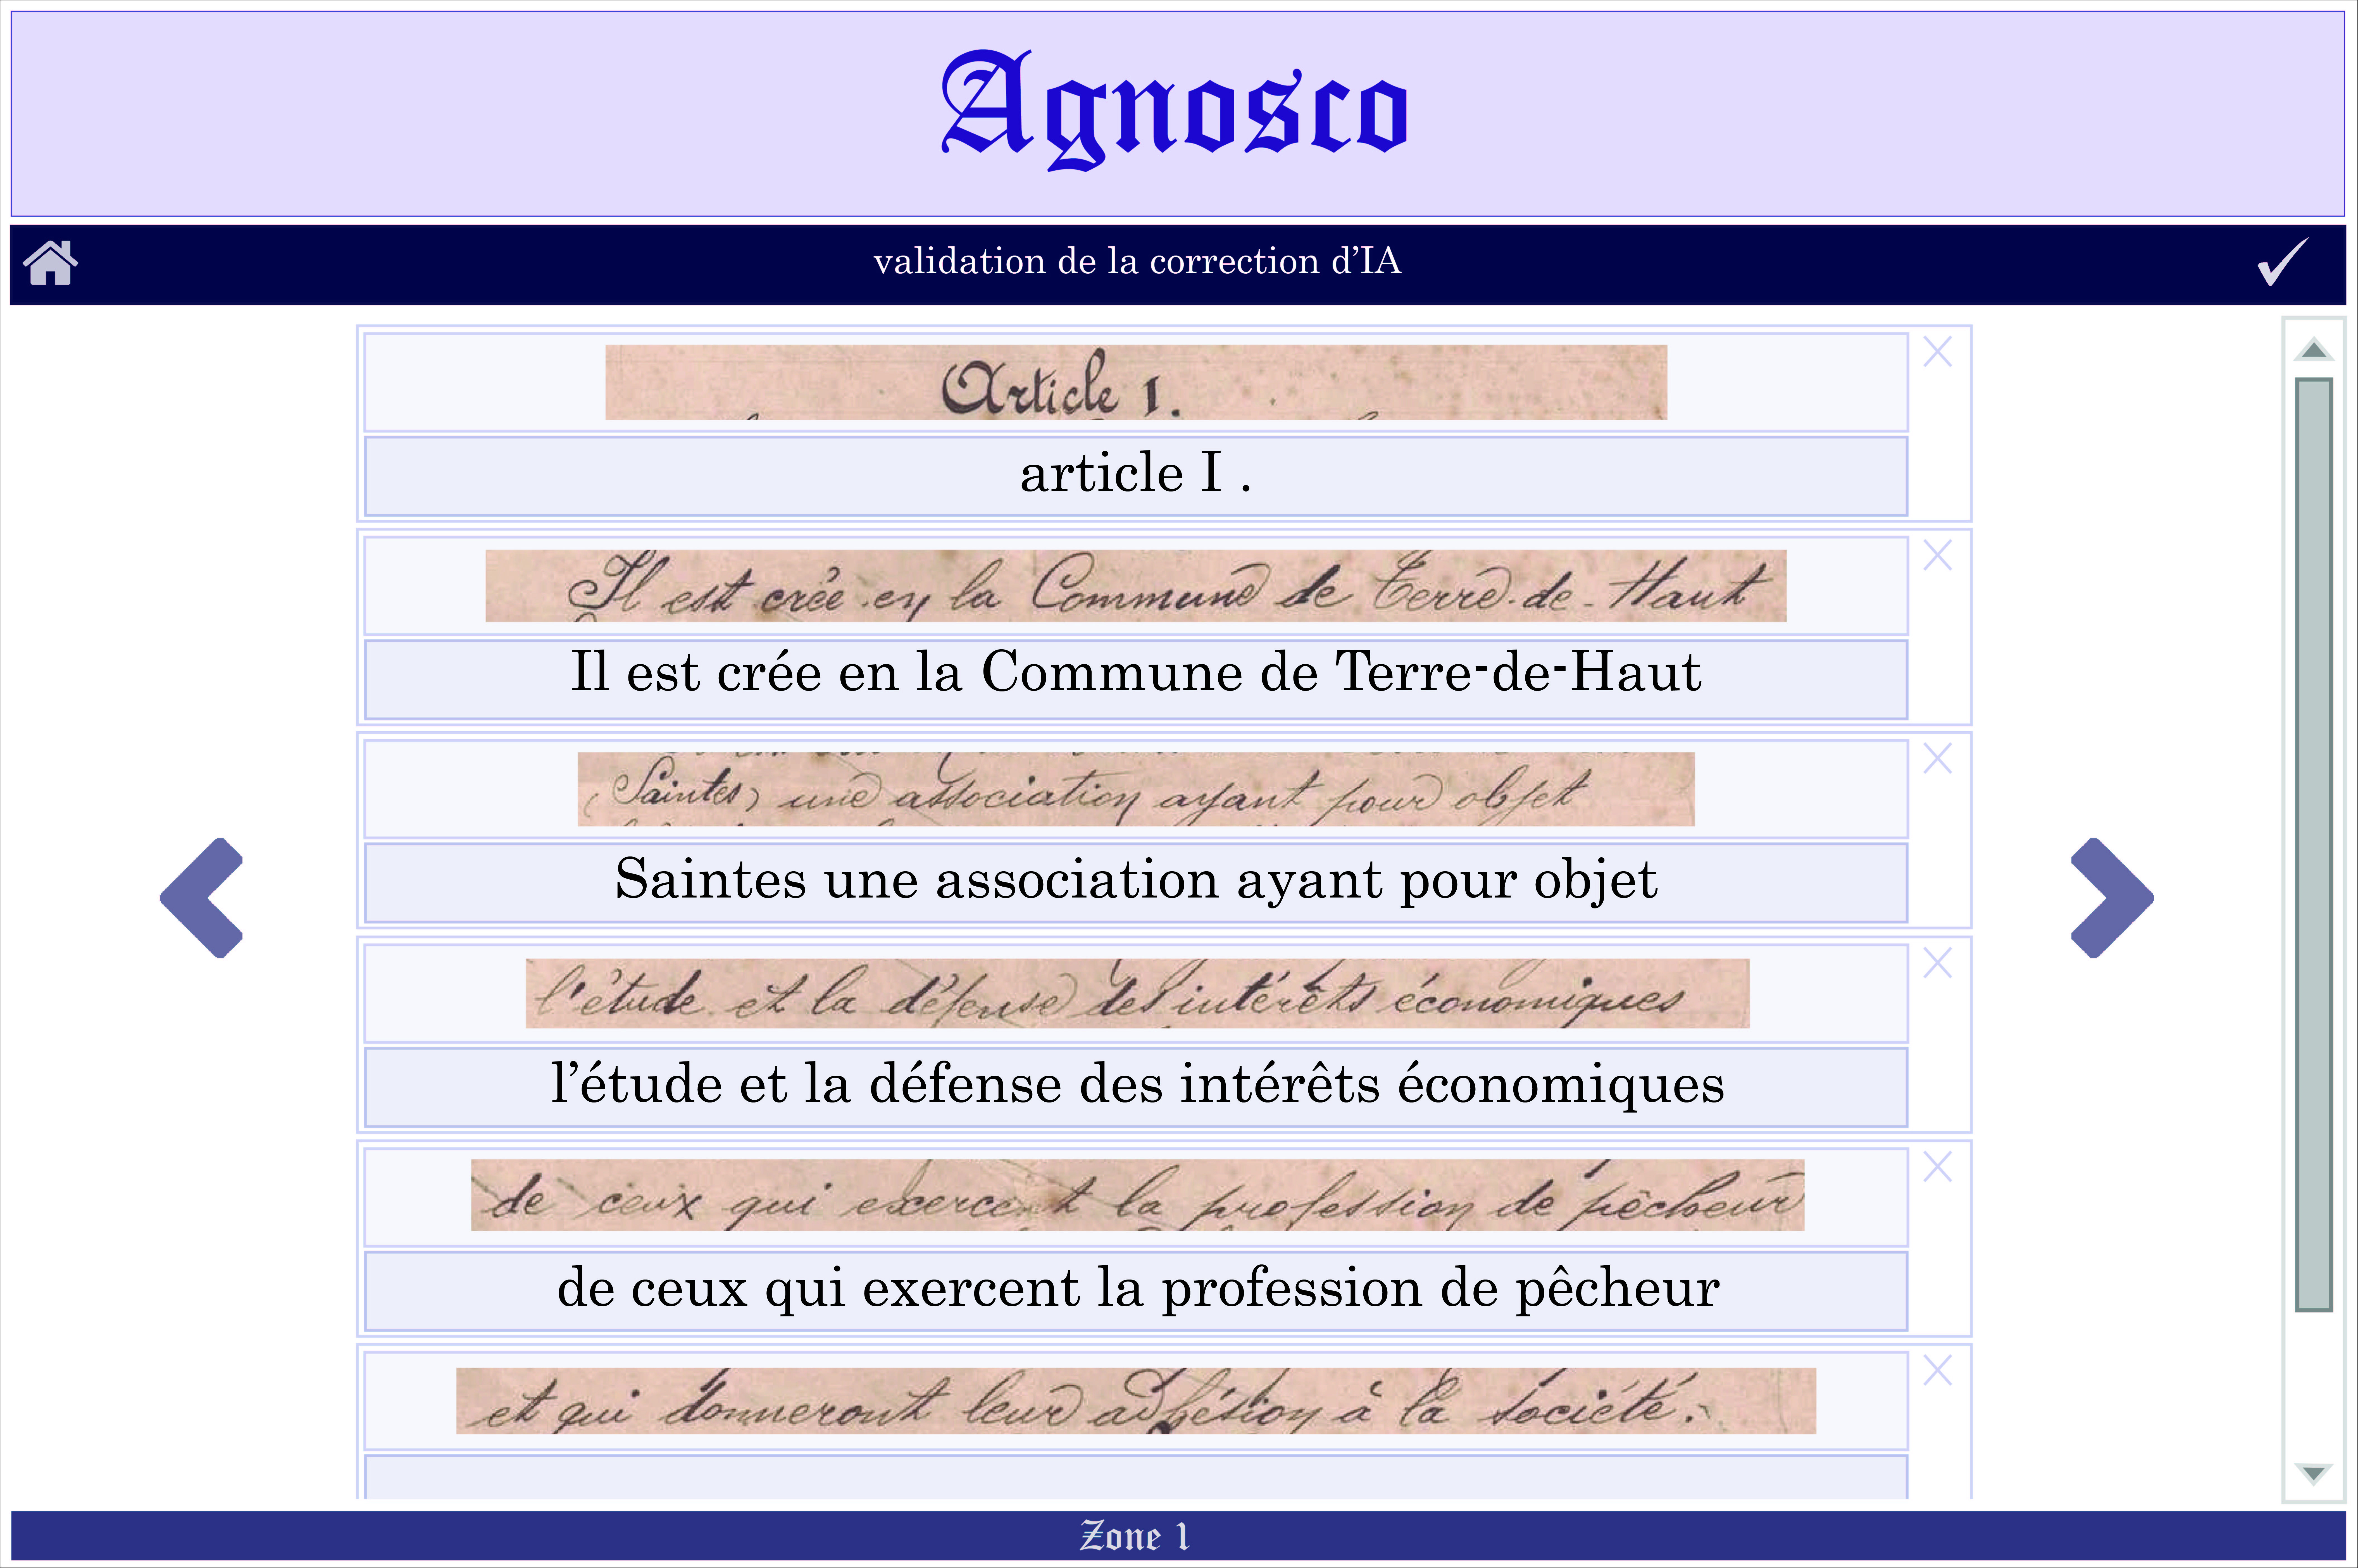
\includegraphics[scale=0.04]{assets/maquetteIHMvalidation1.jpg}
\end{center}
\end{mdframed}

\newpage{}

\paragraph{Deuxième itération}
Pour la deuxième itération, nous implémenterons les fonctionnalités supplémentaires décrites dans les rapports précédents.

\paragraph{}
Nous proposerons tout d’abord une page de découpe des zones ou des paragraphes du document à l’aide d’outils graphiques regroupés dans une zone à droite de la page (spécifications \textit{PDEC\_OD\_1} à \textit{PDEC\_OD\_11}). Il y aura un outil pour créer un nouvelle sélection sous la forme d’un quadrilatère, un outil pour déplacer une sélection existante, un autre pour zoomer et dézoomer, un pour annuler ou refaire la dernière action, un outil pour réinitialiser la découpe et supprimer toutes les sélections réalisées et enfin, un dernier outil “premier jet” permettant de lancer un reconnaisseur de lignes sur les zones découpées. Ce dernier permet de vérifier que les découpes ont bien été réalisées, soit que les lignes sont bien reconnues dans leur intégralité et qu'aucune partie du texte scanné n’est manquante.
\newline{}
La bannière en haut de la page contiendra plusieurs boutons de navigation. Un premier bouton permettra de revenir à l’accueil, comme dans toutes les pages de l’interface. Un autre exportera la page découpée vers un reconnaisseur d’écriture manuscrite en envoyant les couples imagettes - transcriptions au reconnaisseur (\textit{PDEC\_OD\_12}). Tout à droite, un autre bouton permettra à l’utilisateur de passer à la page de transcription manuscrite (\textit{PDEC\_OD\_12}).

\begin{mdframed}[frametitle={Figure 3 : Maquette de la page de découpe des zones}, innerbottommargin=10]
\begin{center}
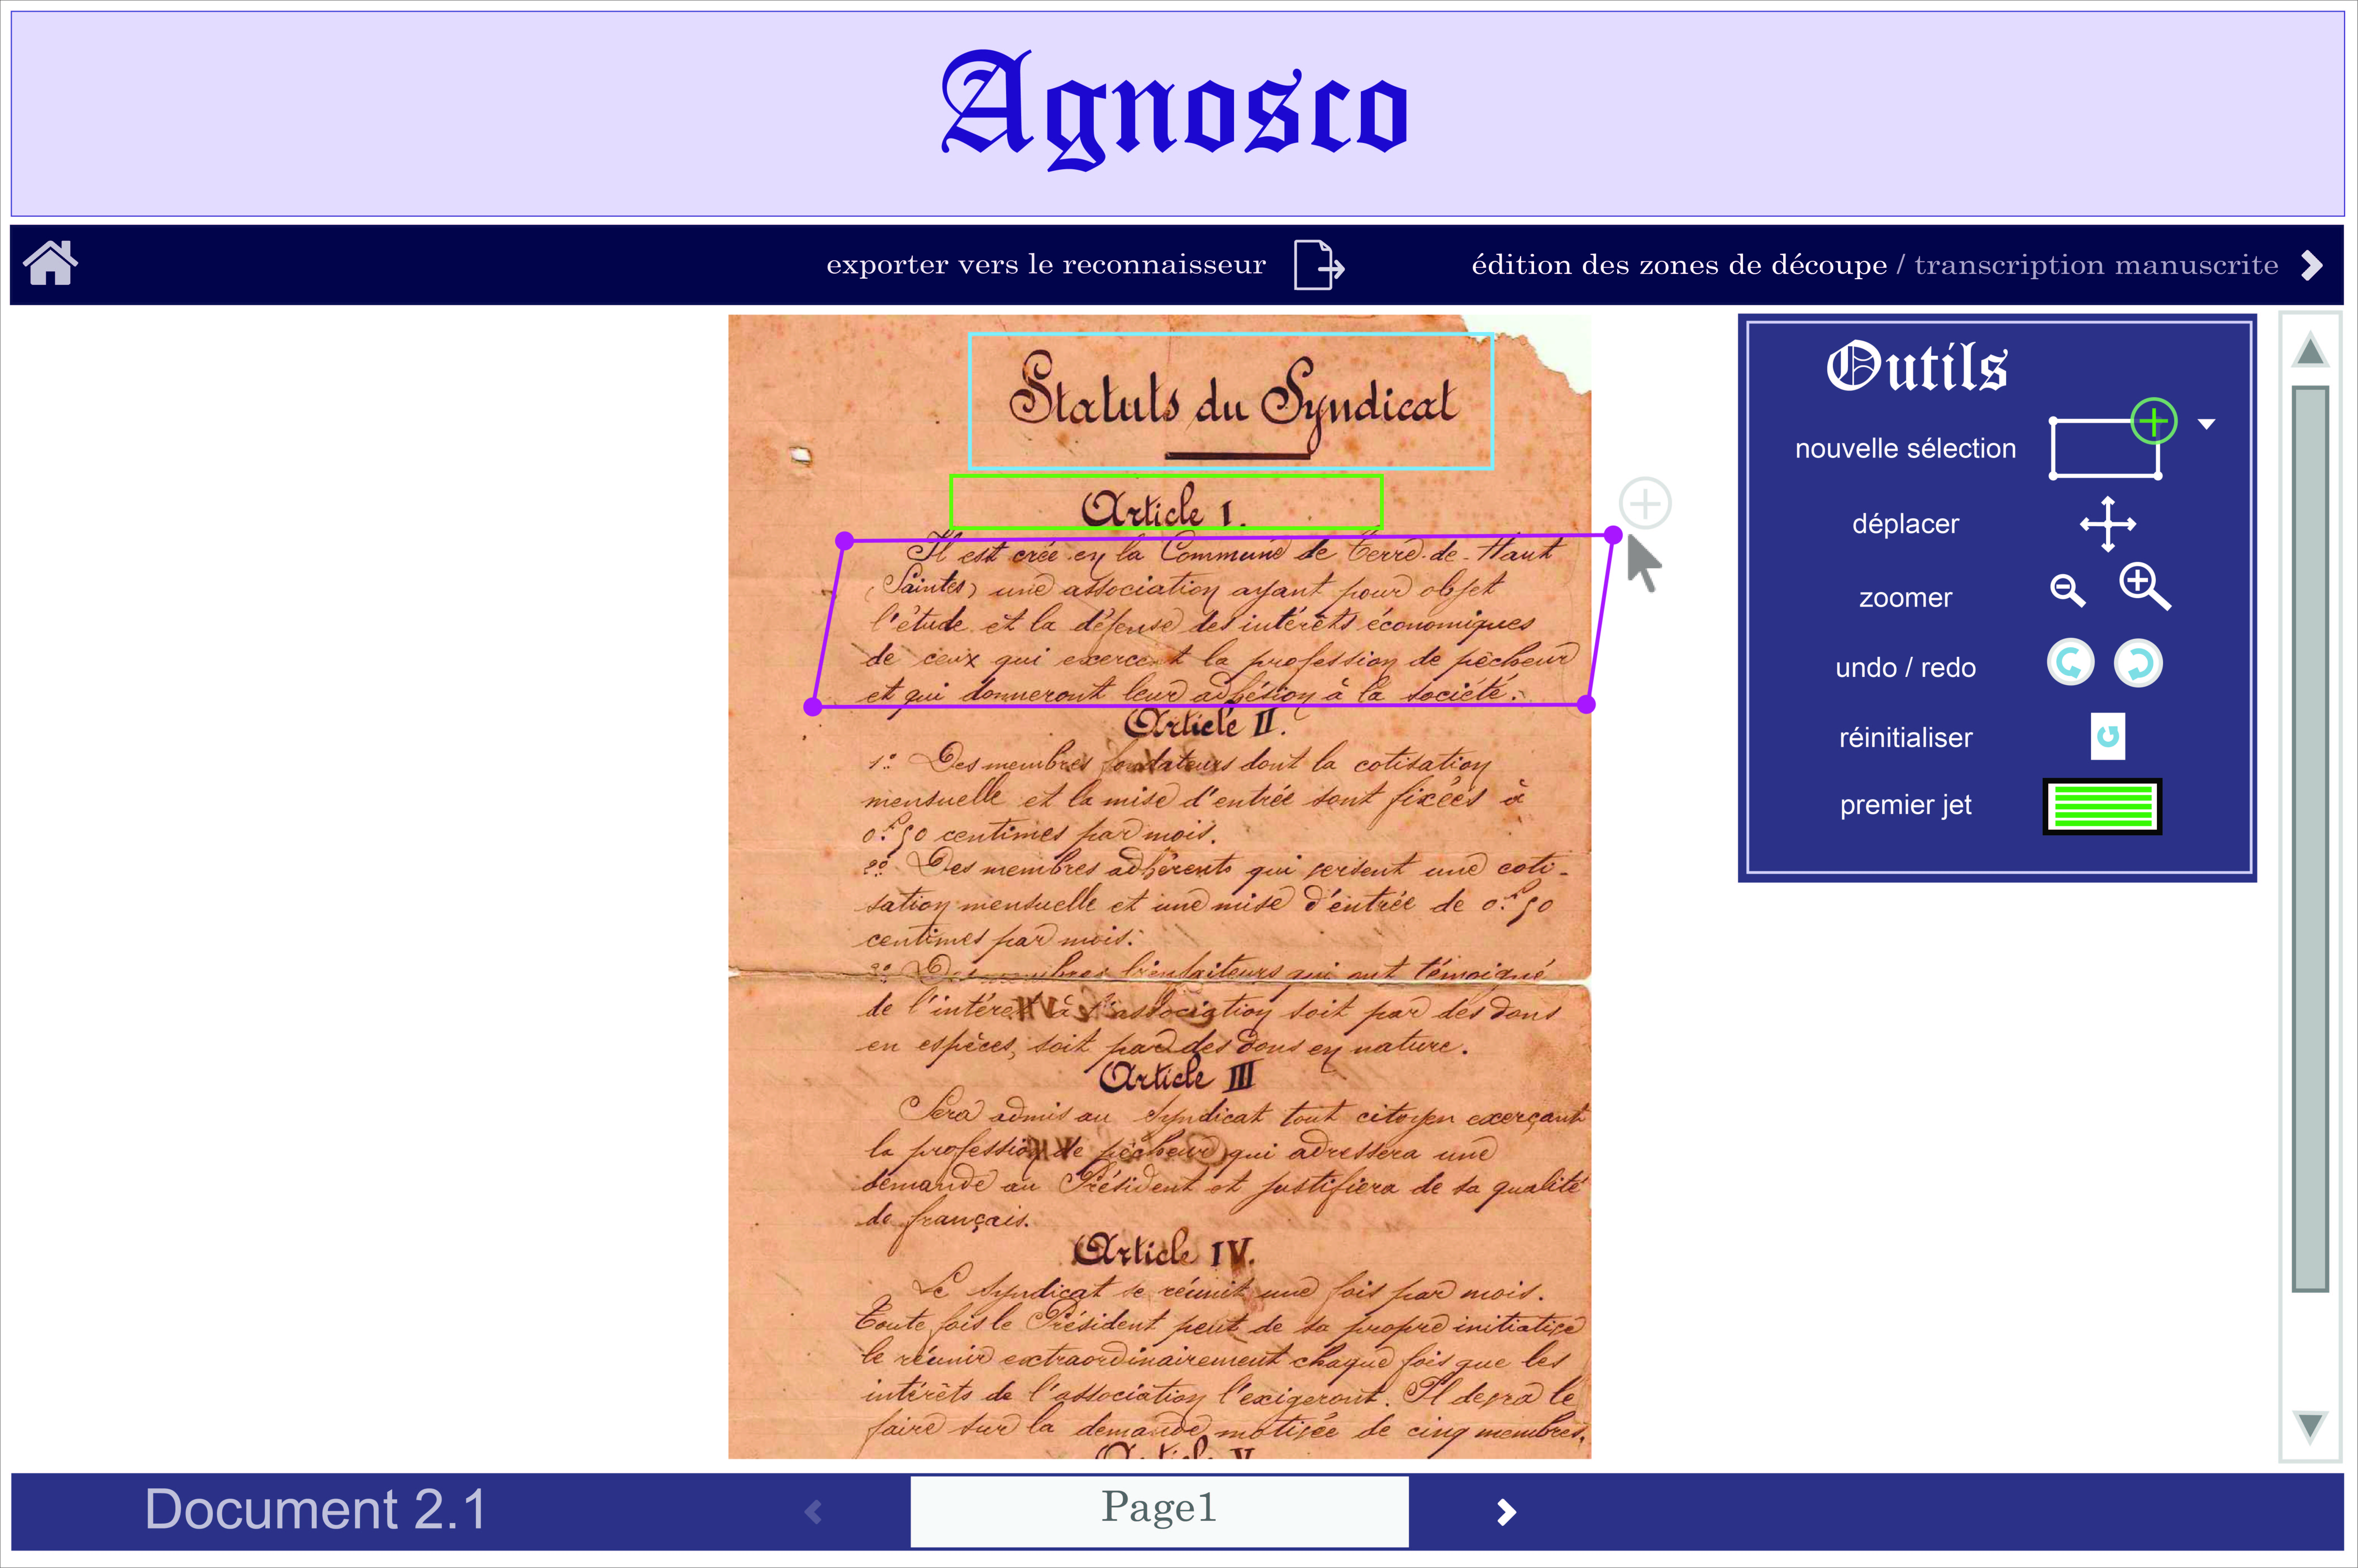
\includegraphics[scale=0.04]{assets/maquetteIHMdecoupes.jpg}
\end{center}
\end{mdframed}

\paragraph{}
Lors de l’ouverture d’un nouveau document de travail, il devra être possible d’utiliser des manuscrits scannés qui ne possèdent pas de vérités-terrain. L’utilisateur aura alors la possibilité d’annoter le manuscrit manuellement ou de le faire passer par un reconnaisseur d’écriture après avoir découpé les zones du manuscrit via la page de découpe de l’interface.

\paragraph{}
L’interface possèdera donc une page d’annotation manuelle (\textit{PEA\_GEN\_2}). Les imagettes d’une même zone seront affichées à la suite dans la fenêtre centrale, avec une zone de texte pour la transcription située sous chaque imagette. Le curseur sera positionné automatiquement sur la première transcription affichée (\textit{PEMA\_1}), l’utilisateur devra taper la transcription manuellement au clavier puis appuyer sur la touche \texttt{Entrée} pour passer à la transcription suivante (\textit{PEMA\_2}). Lorsque toutes les imagettes d’une zone ont été annotées, on passe automatiquement aux imagettes de la zone suivante à l’appui sur \texttt{Entrée} de la dernière transcription. Le but est de minimiser les actions requises par l’utilisateur, pour qu’il n’utilise que son clavier. Il peut néanmoins positionner son curseur sur la transcription de son choix à l’aide de sa souris.
\newline{}
Une croix à droite de chaque imagette permet de supprimer le couple imagette-transcription de la base d’apprentissage si le couple est jugé peu pertinent (\textit{PEMA\_6}). Après l’appui sur ce bouton, le couple est flouté mais toujours visible et la croix est remplacée par une flèche montante qui permet de réintroduire le couple supprimé dans la base d’apprentissage.
\newline{}
Cette page de l’interface possèdera également une fenêtre à droite montrant la page courante en entier, avec toutes ses zones de découpe affichées en surbrillance. Un rectangle parcourera la page au fur et à mesure de la transcription pour indiquer la position courante dans la page.
\newline{}
Sous cette fenêtre de visualisation de la page, l’interface proposera une fenêtre de navigation dans les différents documents, permettant à l’utilisateur d’ouvrir un autre document de travail à tout moment.
\newline{}
Dans la bannière en haut de la page, un bouton permettra à l’utilisateur de revenir à la page de découpe des zones ou encore d’avancer à la page de validation finale des transcriptions, tandis qu’un autre renverra à l’accueil.

\begin{mdframed}[frametitle={Figure 4 : Maquette de la page d'annotation manuelle}, innerbottommargin=10]
\begin{center}
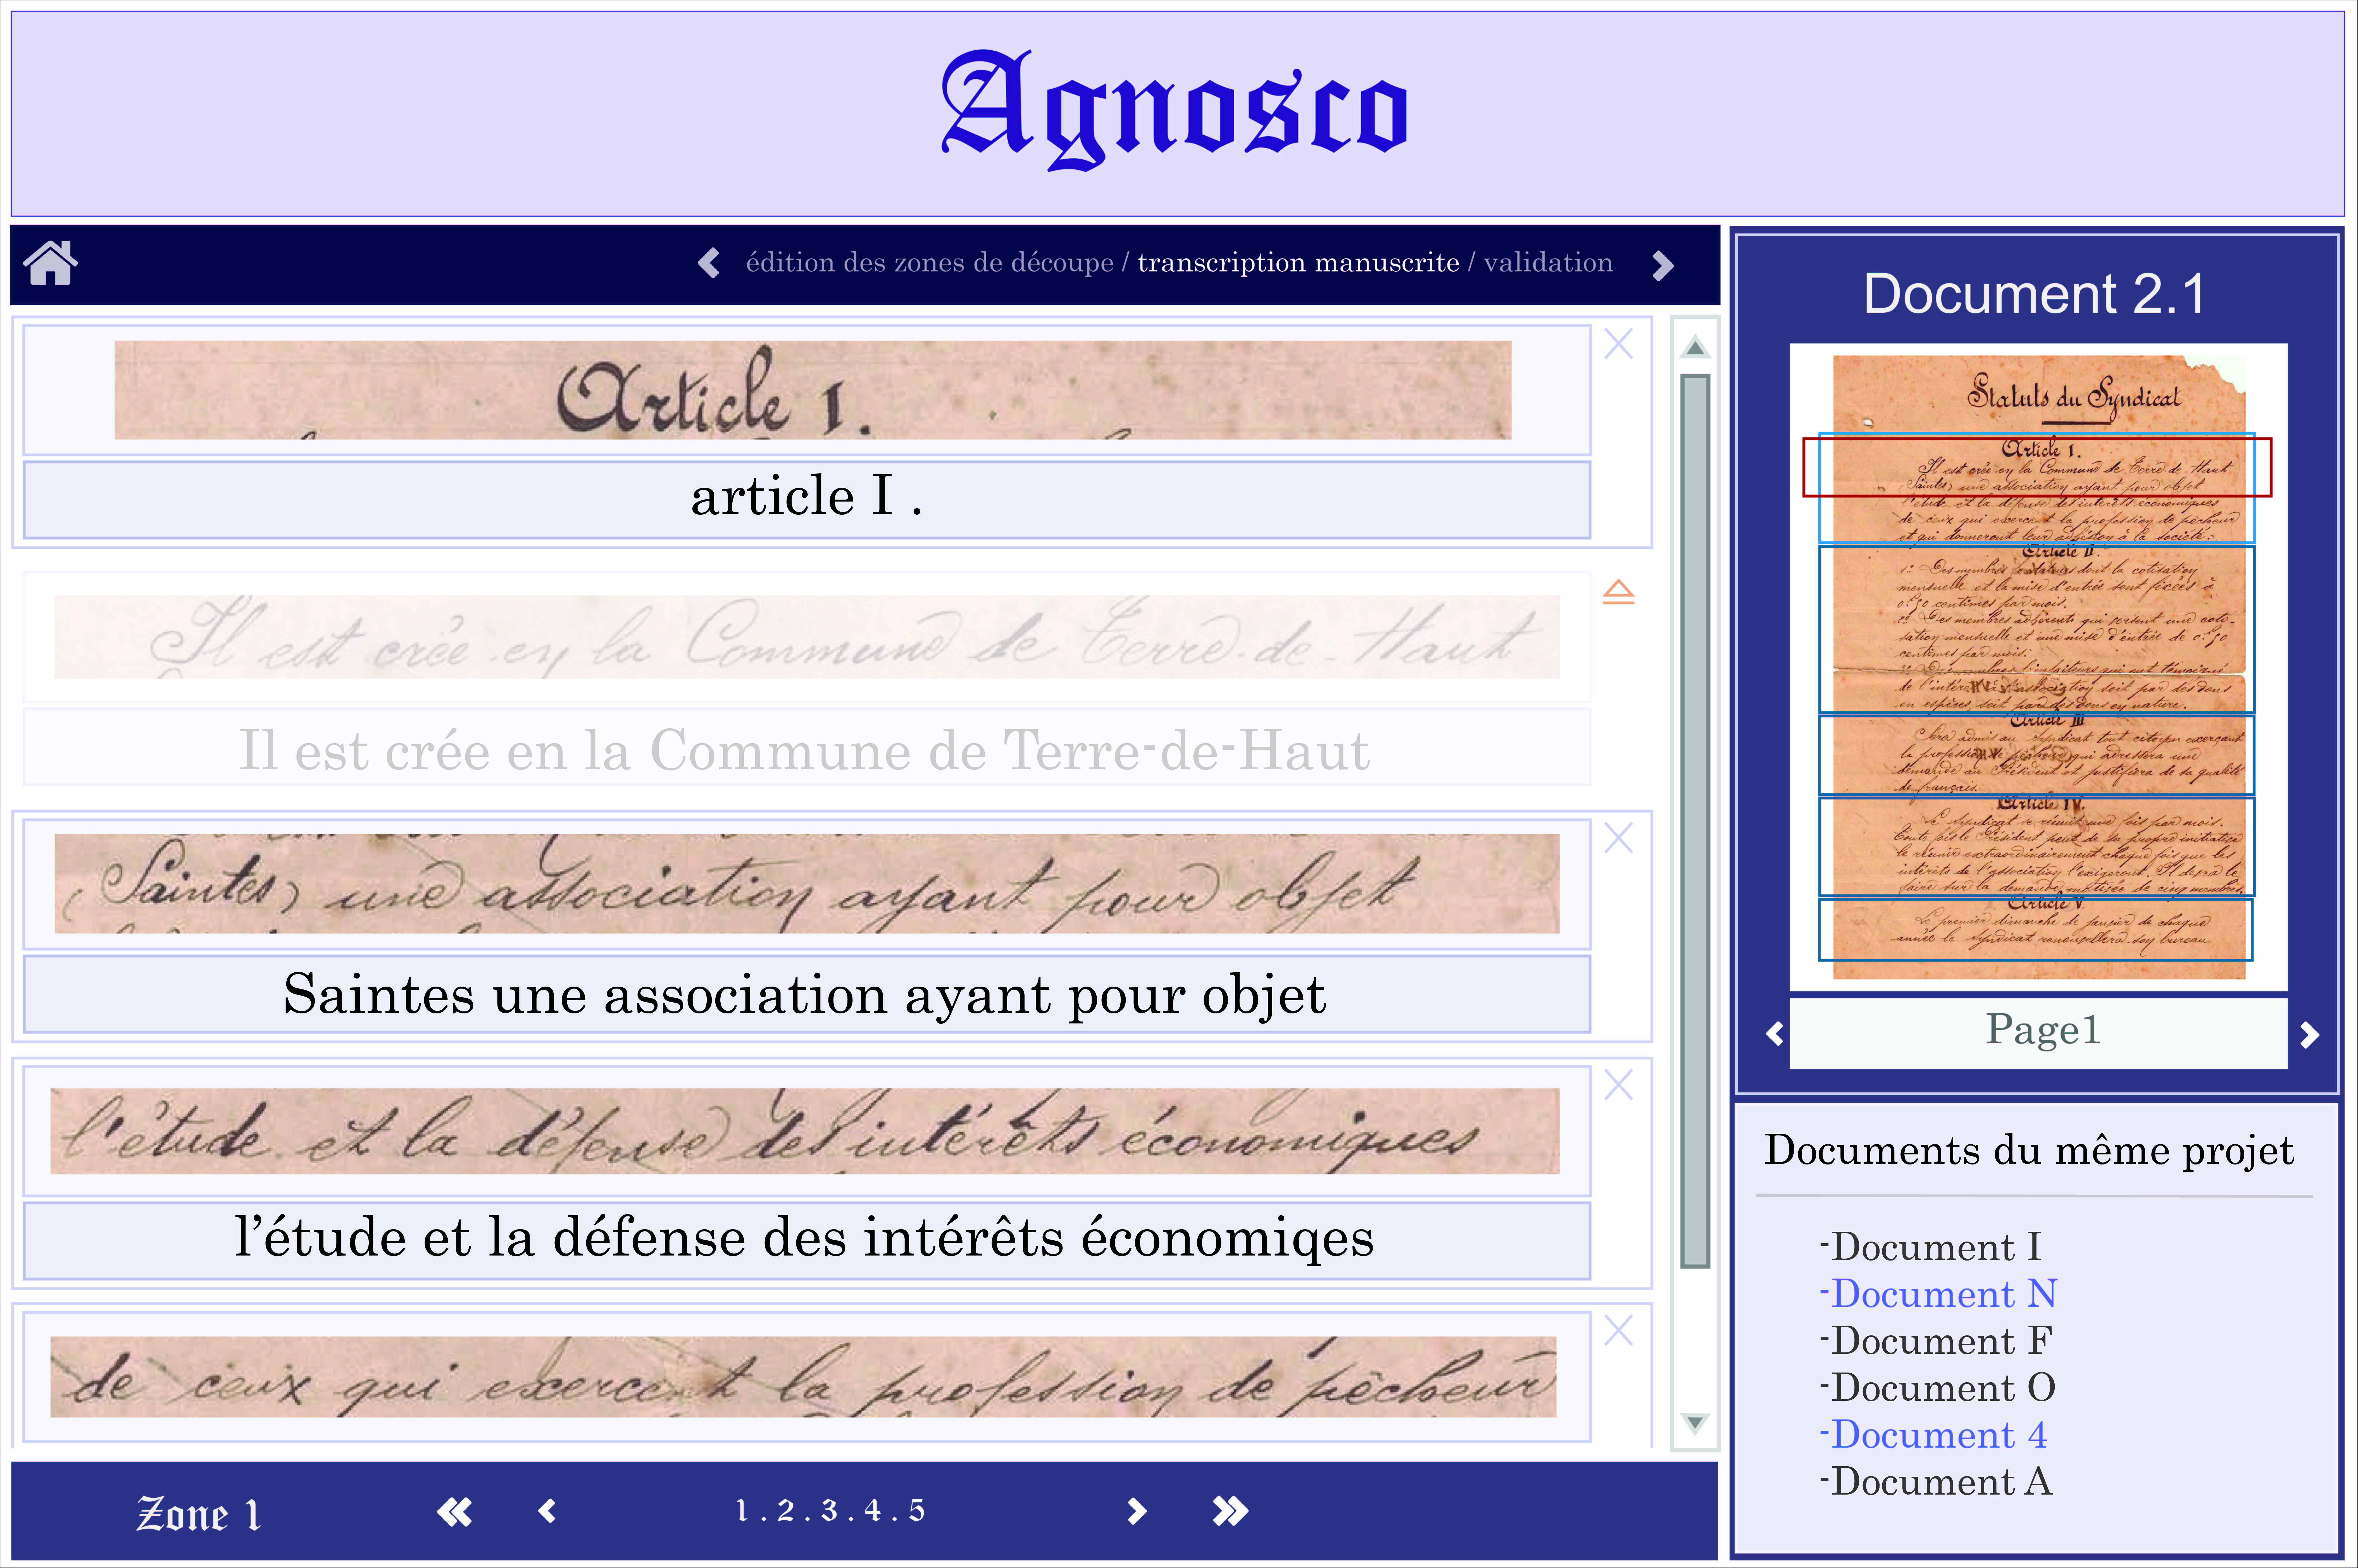
\includegraphics[scale=0.04]{assets/maquetteIHMtranscriptionmanu.jpg}
\end{center}
\end{mdframed}

\paragraph{}
Si l’utilisateur souhaite faire passer le manuscrit par le reconnaisseur plutôt que de l’annoter manuellement, il pourra visualiser et corriger les résultats de la reconnaissance via la page dédiée de l’interface (\textit{PEA\_GEN\_3}). Cette page sera sensiblement similaire à la page d’annotation manuelle, la différence principale résidant dans le fait que des transcriptions réalisées par le reconnaisseur seront déjà présentes sous chaque imagette. Le curseur se positionnera automatiquement sur la première transcription et un simple appui sur la touche \texttt{Entrée} passera à la transcription suivante. L’utilisateur pourra modifier manuellement la transcription courante en tapant ses modifications au clavier (spécifications \textit{PCORIA\_1} à \textit{PCORIA\_5}).
\newline{}
Dans la bannière du haut de la page, un bouton renverra à l’accueil et un autre permettra la navigation vers la page de validation finale des transcriptions.

\newpage{}

\begin{mdframed}[frametitle={Figure 5 : Maquette de la page de visualisation des transcriptions du reconnaisseur}, innerbottommargin=10]
\begin{center}
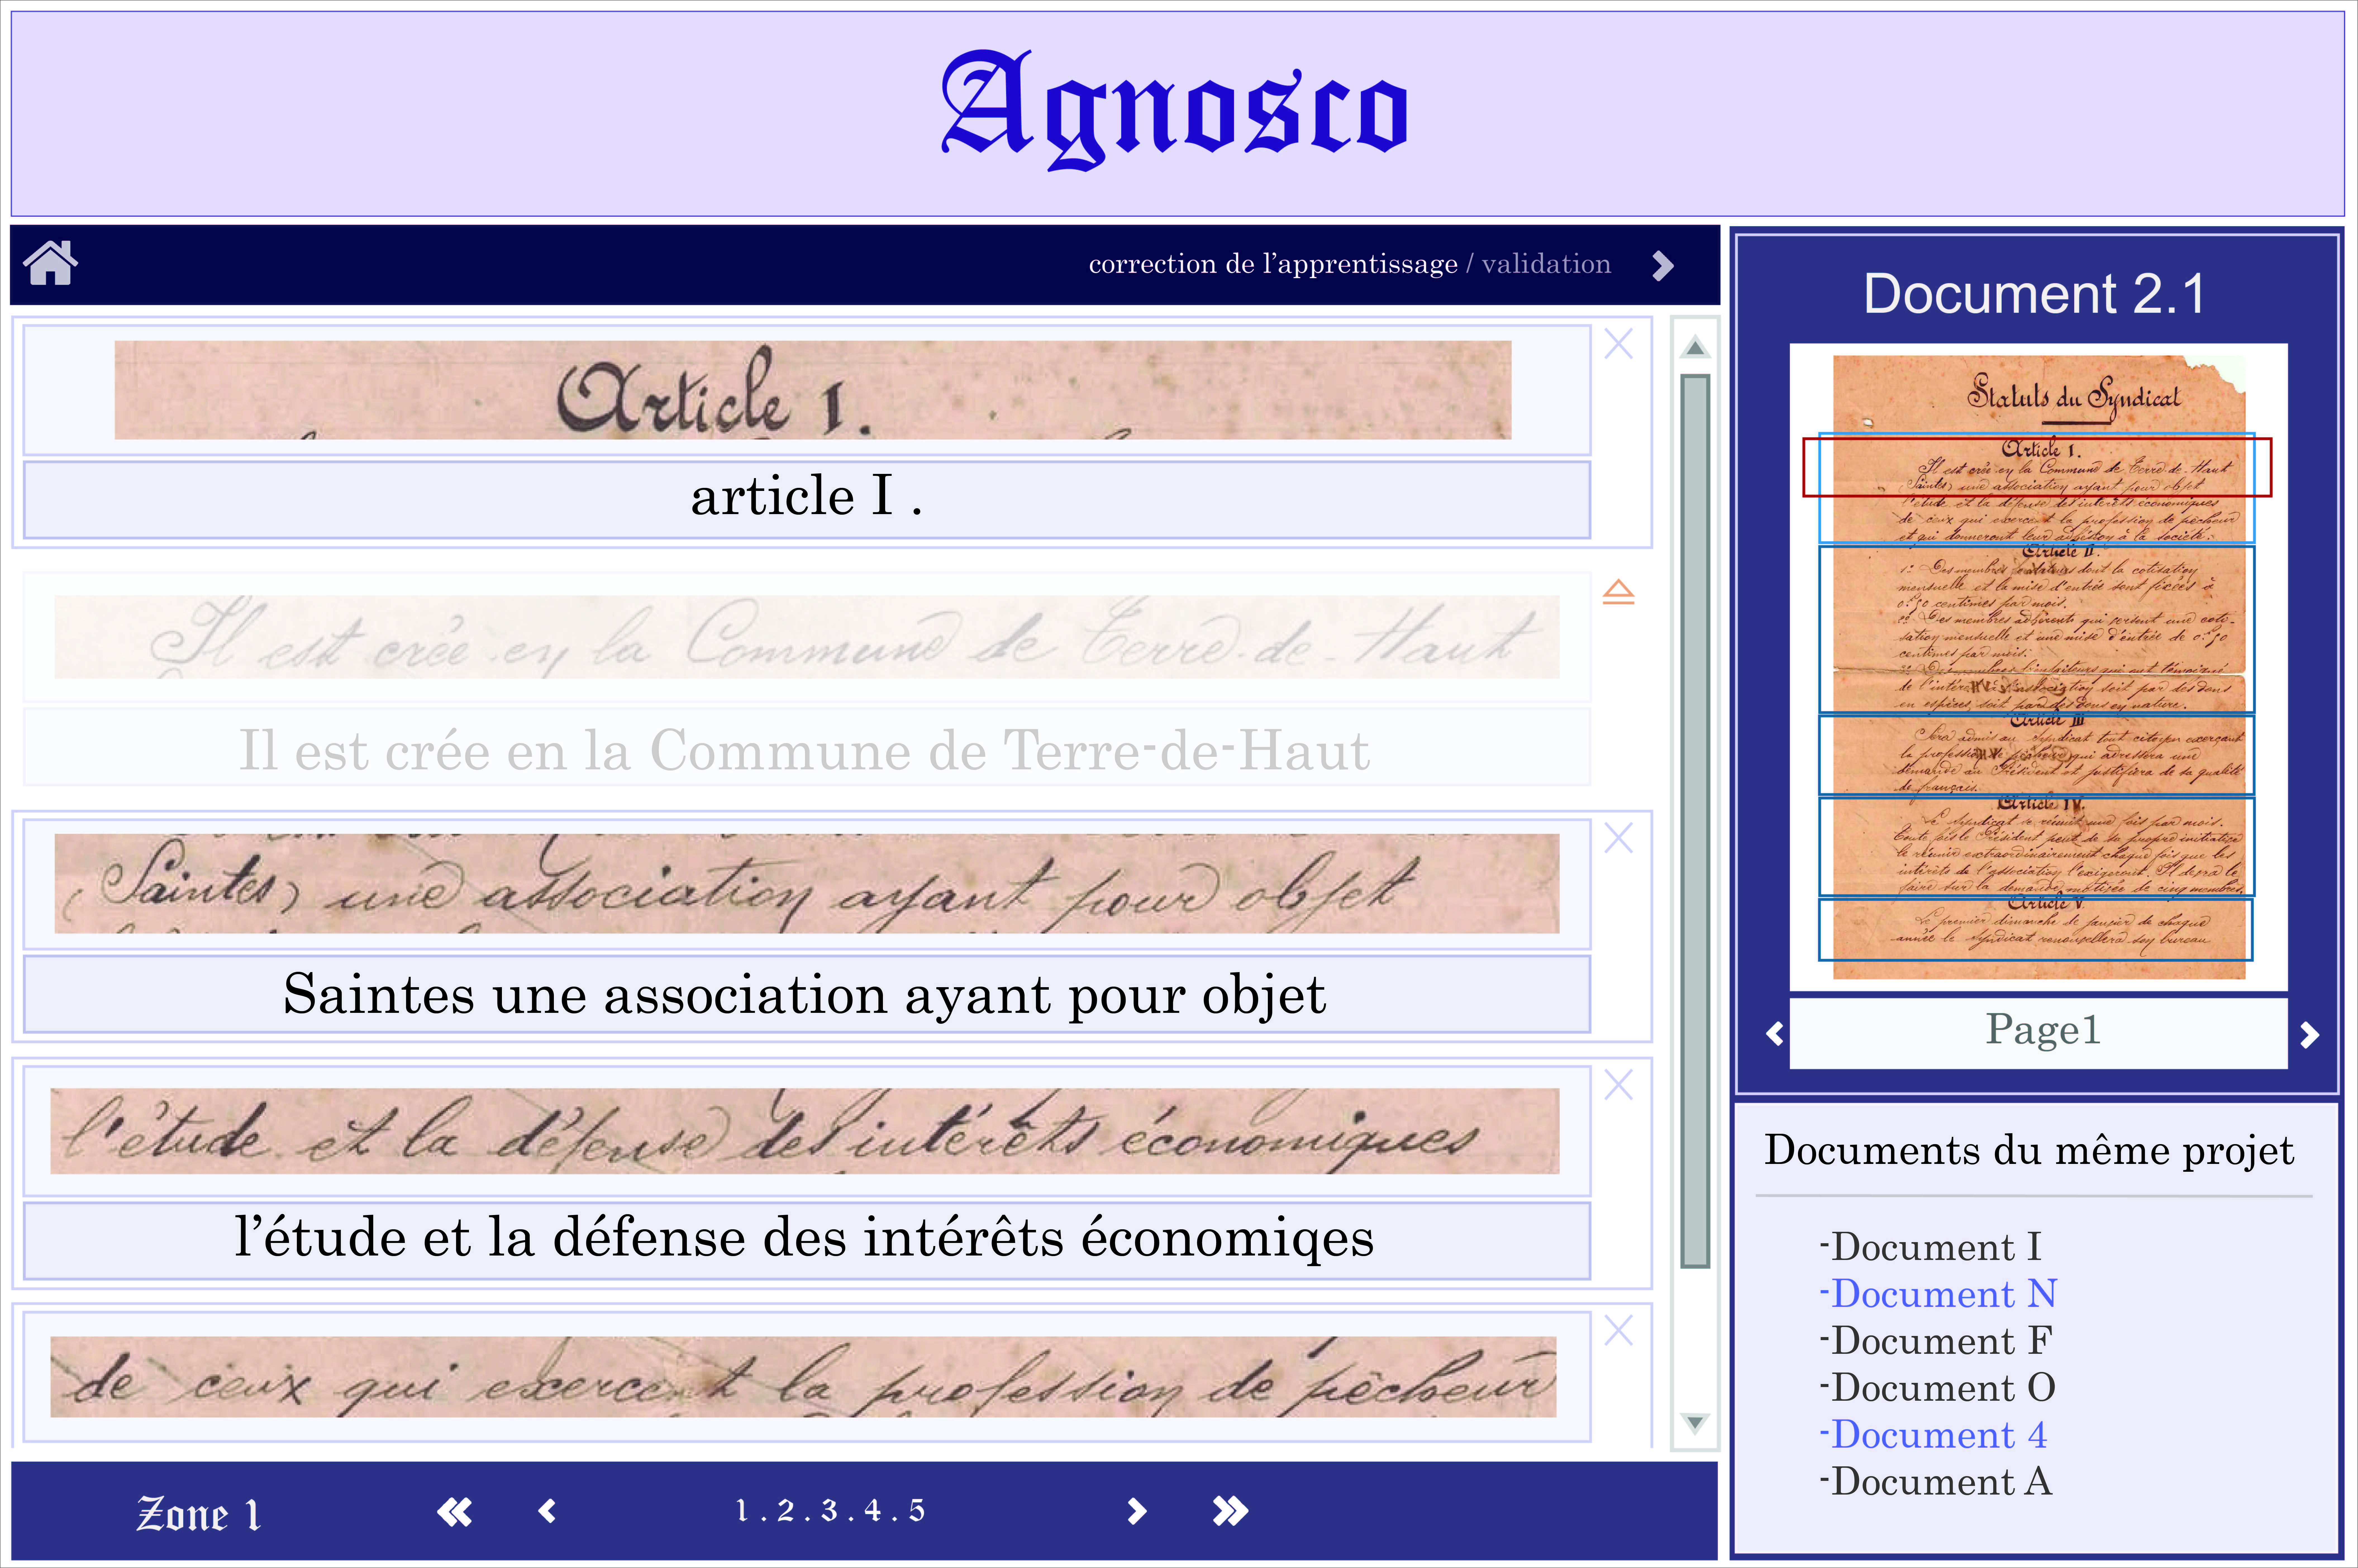
\includegraphics[scale=0.04]{assets/maquetteIHMcorrectionIA.jpg}
\end{center}
\end{mdframed}

\paragraph{}
Enfin, la dernière page de l’interface sera la page de validation qui a déjà été réalisée lors de la première itération. Deux modifications y seront apportées pour la deuxième itération.
\newline{}
Tout d'abord, une fenêtre sera ajoutée pour visualiser la page courante en miniature avec ses zones de découpe affichées par dessus ainsi qu’un rectangle montrant la position courante de l’utilisateur, afin que ce dernier ait constamment accès à sa position dans le document.
\newline{}
Ensuite, la bannière en haut de la page affichera si les transcriptions ont été réalisées manuellement par un humain ou par le reconnaisseur d'écriture, car l'attention fournie par l'utilisateur devrait être moindre pour un manuscrit annoté manuellement où les fautes sont théoriquement moins nombreuses. Savoir si la transcription a été faite manuellement ou par le reconnaisseur permettrait d'augmenter la rapidité de la validation finale.

\begin{mdframed}[frametitle={Figure 6 : Maquette de la page de validation finale lors de la deuxième itération}, innerbottommargin=10]
\begin{center}
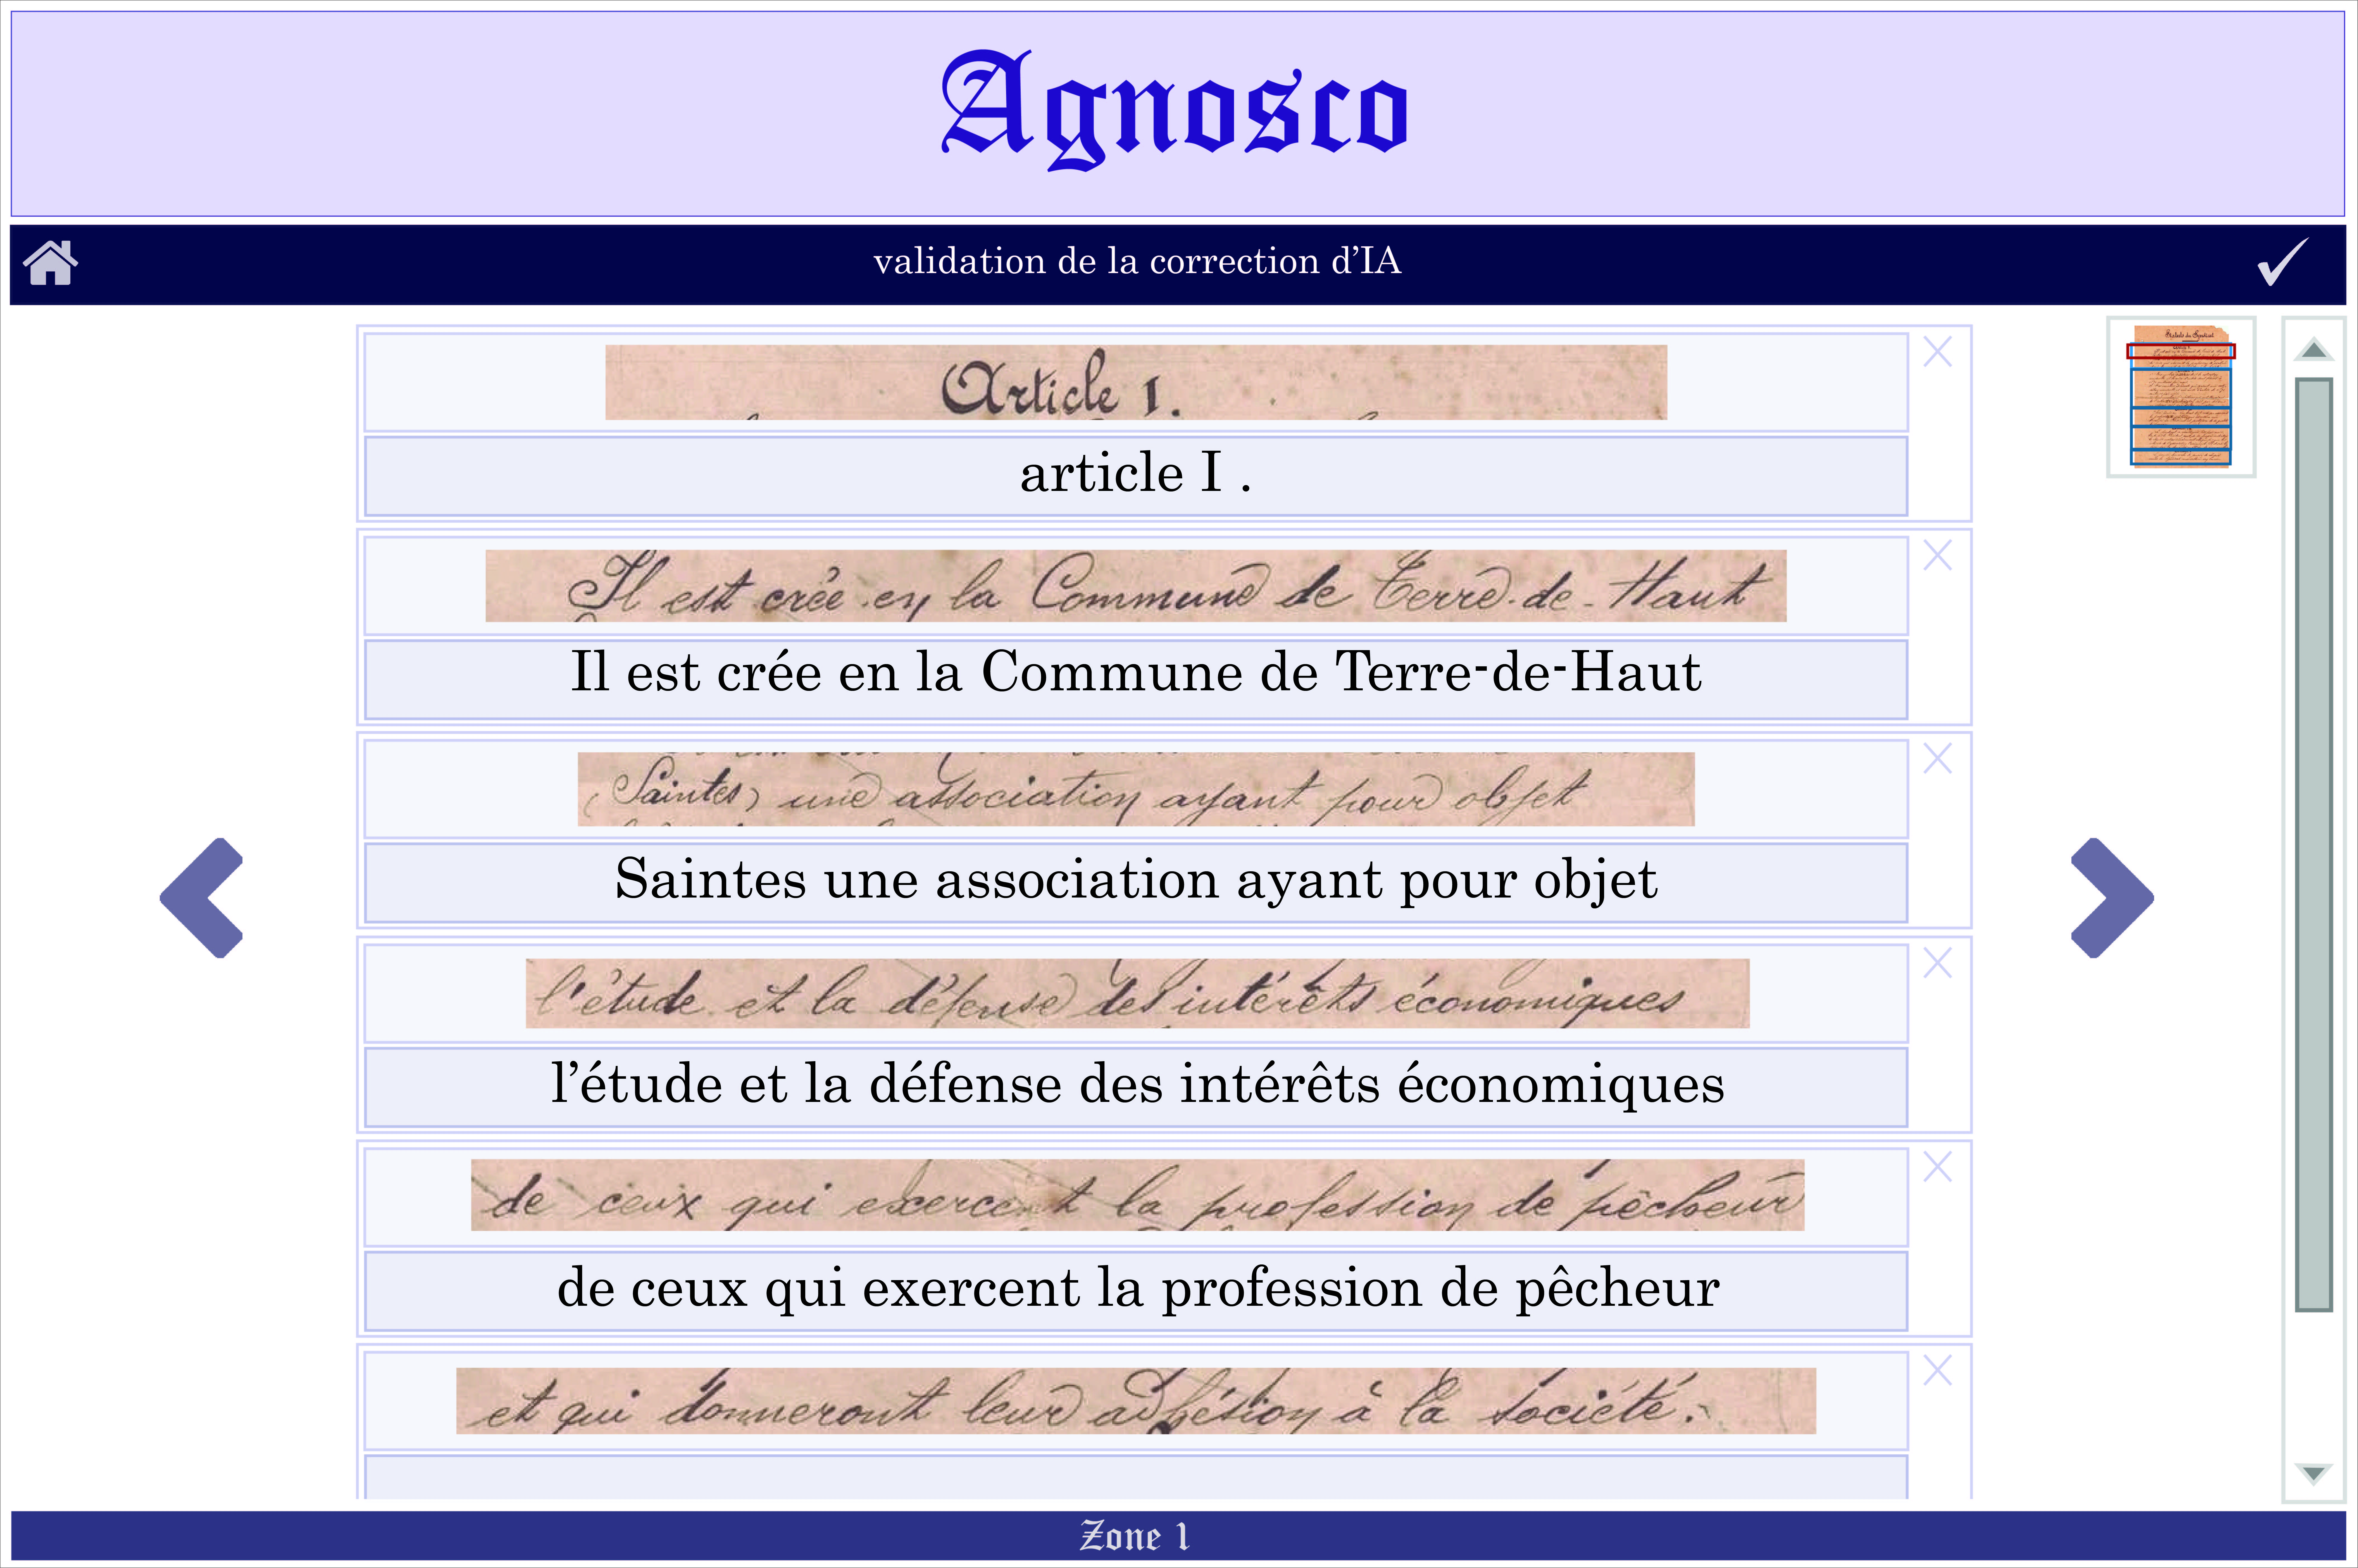
\includegraphics[scale=0.04]{assets/maquetteIHMvalidationIA.jpg}
\end{center}
\end{mdframed}

\paragraph{}
En résumé, à la fin de la deuxième itération, nous aurons cinq composants différents : la page d’accueil, la page de découpe des zones du document, la page d’annotation manuelle, la page de visualisation de la reconnaissance et la page de validation finale des transcriptions.


%-------------------------------------------------------------------------------
\section{Interactions}

\paragraph{Interactions entre les composants de l'interface}
L’utilisateur peut naviguer entre les différents composants via les boutons de l’interface.
\newline{}
Tout d’abord, une icône permettant de revenir à la page d’accueil sera présente en haut à gauche de chaque page - à l’exception de la page d’accueil. Sur cette dernière, le choix du document ouvre celui-ci dans la page de l’interface qui lui correspond, soit :

\begin{itemize}
\item la page de découpe si aucun travail n’a été réalisé au préalable sur ce document ;
\item la page d’annotation manuelle si les découpes ont déjà été réalisées et que l’utilisateur n’a pas exporté le document vers le reconnaisseur ;
\item la page de visualisation des transcriptions du reconnaisseur si une reconnaissance a été réalisée sur le document ;
\item ou la page de validation finale si toutes les transcriptions ont déjà été renseignées.
\end{itemize}

Des boutons de navigation dans les différentes pages sont également présents sur certaines pages, comme décrit dans la partie précédente. Les interactions sont visibles dans le schéma ci-dessous :

\begin{mdframed}[frametitle={Figure 7 : Schéma des interactions entre les différents composants de l'IHM}, innerbottommargin=10]
\begin{center}
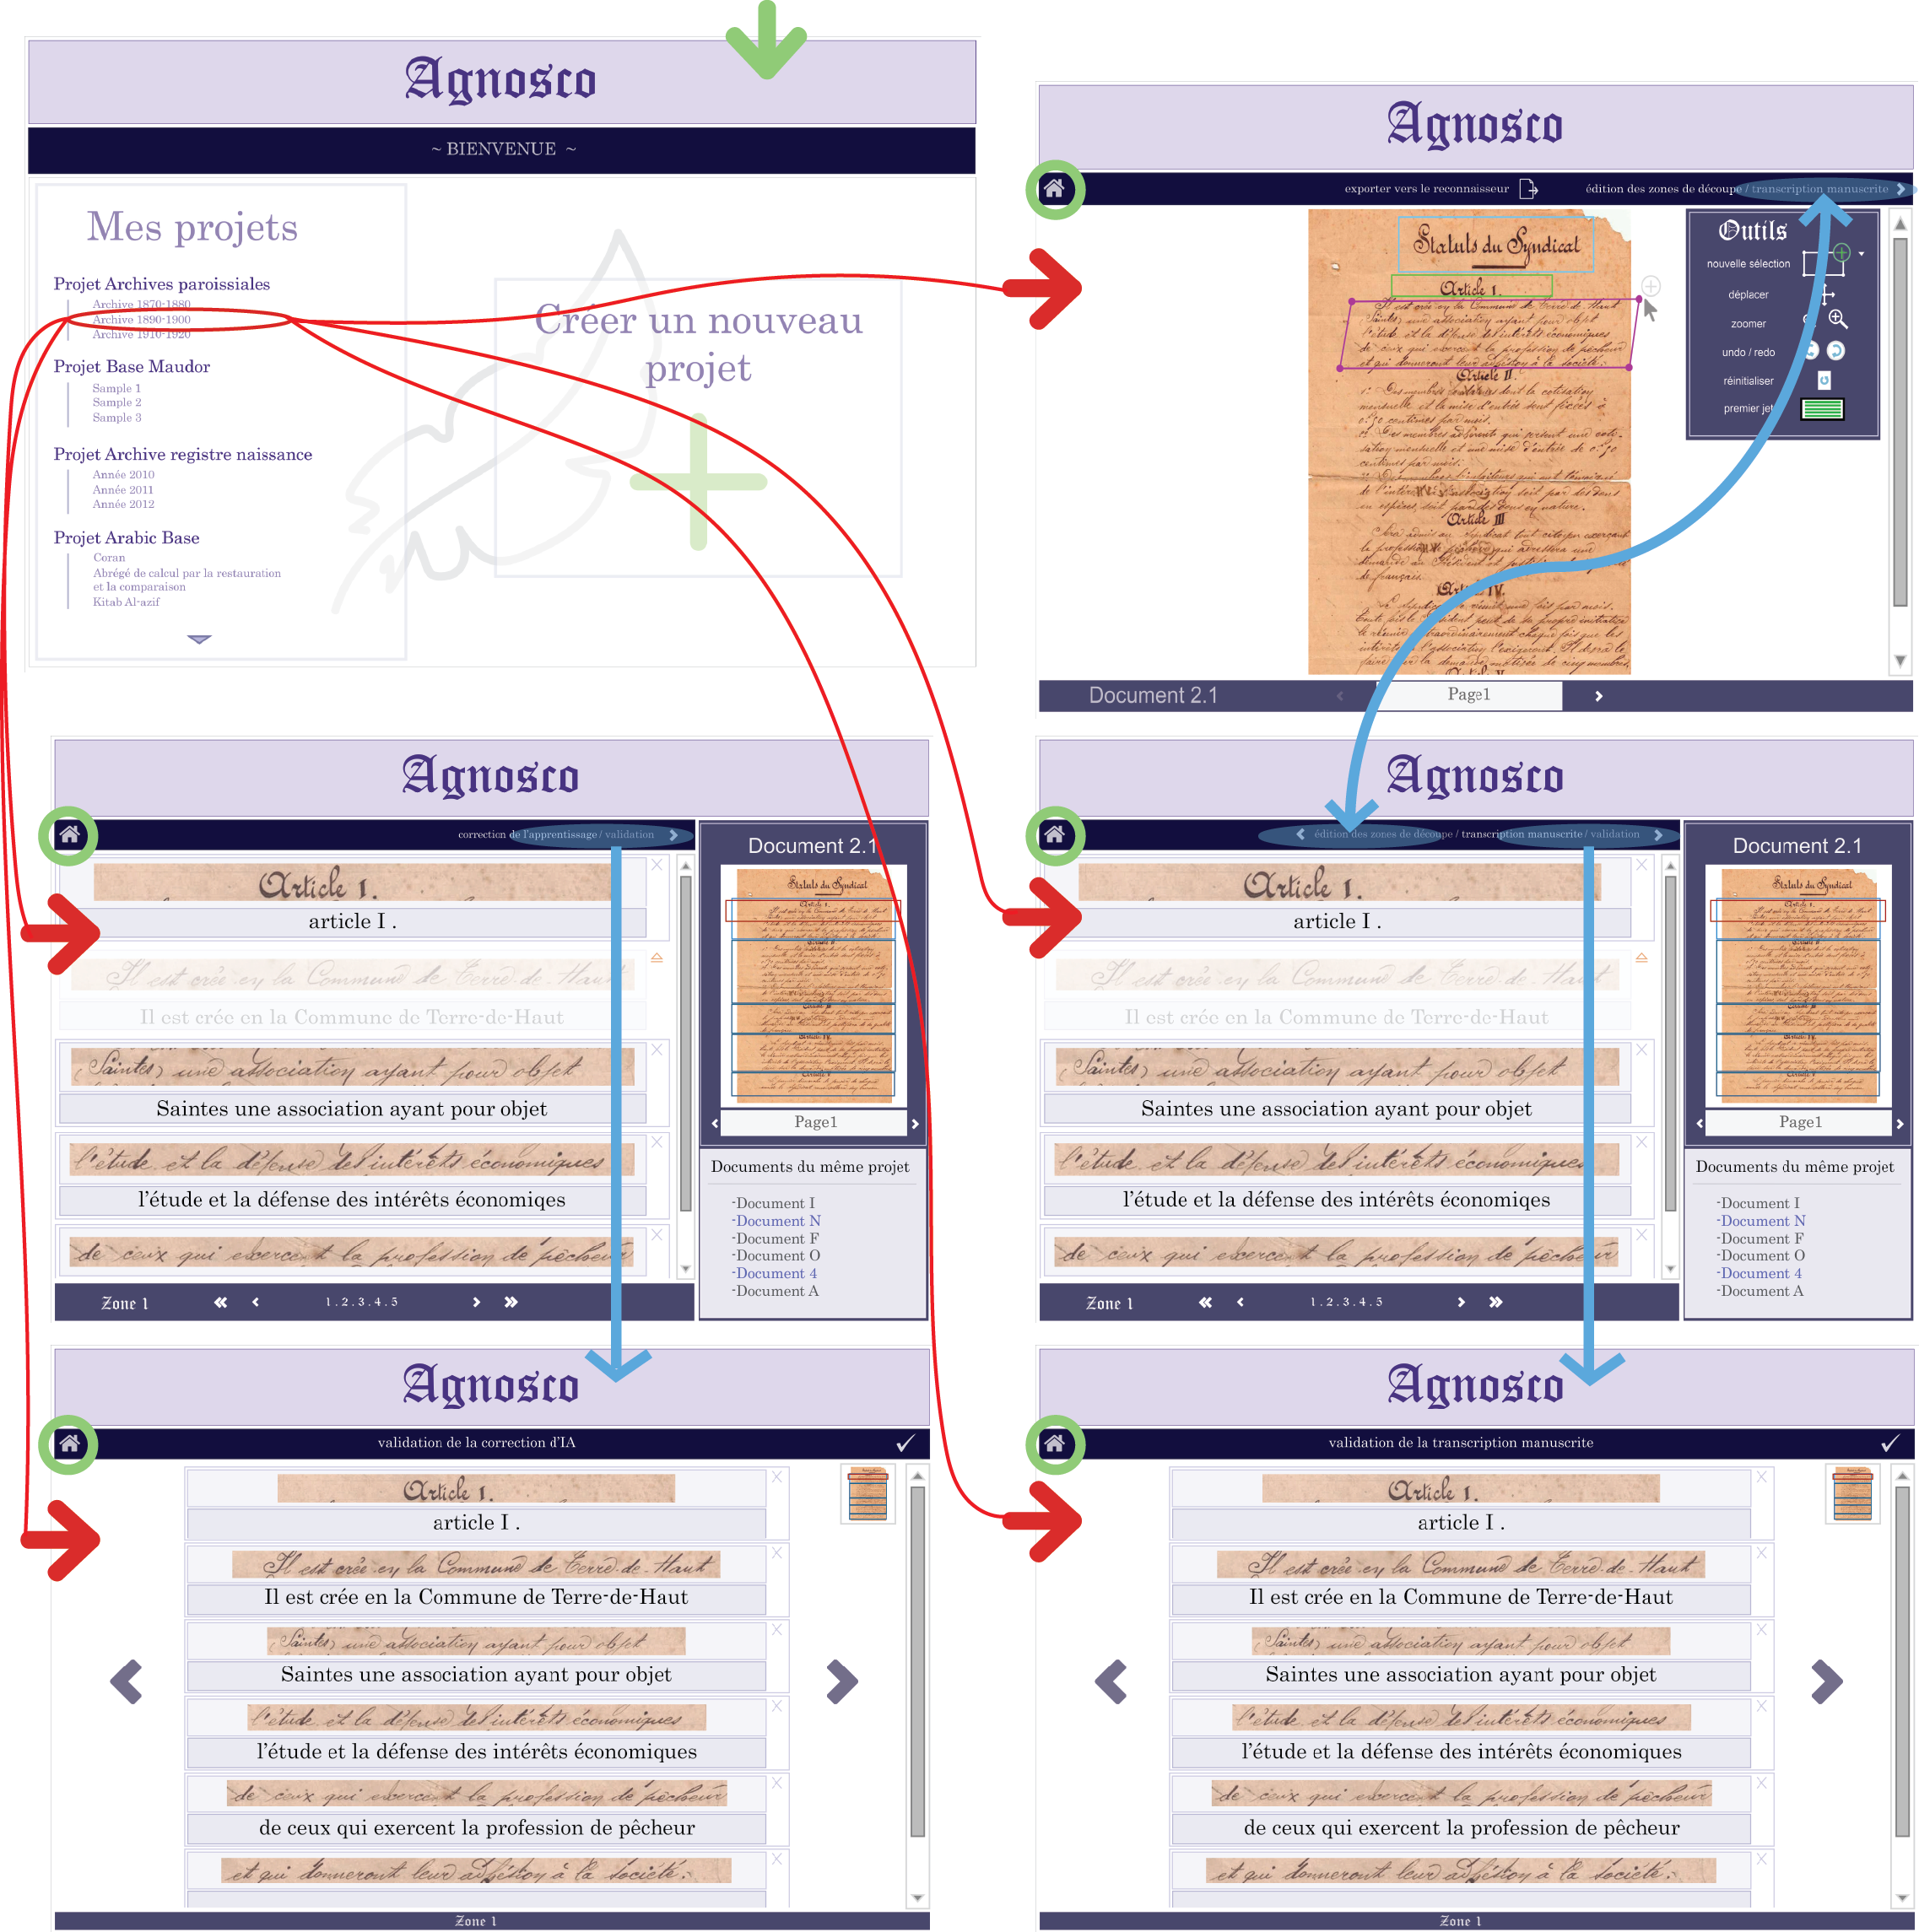
\includegraphics[scale=0.5]{assets/schemaIHMinteractions.png}
\end{center}
\end{mdframed}

\paragraph{Interactions entre le \textit{front-end} et le \textit{back-end}}

L’interface affiche les informations de la base de données (les couples imagettes - transcriptions) et les modifie. Pour ce faire, elle est reliée au connecteur central via sa ressource Rest. Le connecteur traite les demandes de l’IHM et les envoie au connecteur de la base de données. Celui-ci effectue les ordres de l’utilisateur sur la base et renvoie les imagettes et les transcriptions au connecteur central qui les fait suivre à l’IHM. Les modifications (ajout ou modification d’une transcription ou suppression d’un couple) sont enregistrées localement puis envoyées à la base de données lors du changement de page et du chargement d'une nouvelle page. Nous n'avons donc pas de bouton spécifique pour enregistrer les modifications.

\newpage{}

\paragraph{API Rest}
Pour communiquer avec le \textit{back-end}, nous utiliserons une API \texttt{Rest} dont les requêtes sont listées ci-dessous.
\newline{}

\begin{description}[align=left]

\item [Général]

\item [GET] \texttt{/base/projectsAndDocuments}\newline{}
\begin{itshape}
Renvoie la liste des noms des projets, contenant pour chaque projet une liste des noms des documents qui le composent.
\end{itshape}

\item [DELETE] \texttt{/base/deleteDocument/\{name\}}\newline{}
\begin{itshape}
Supprime le document de la base qui porte le nom donné, ainsi que son contenu.
\end{itshape}

\item [GET] \texttt{/base/availableRecognisers}\newline{}
\begin{itshape}
Renvoie la liste des noms des reconnaisseurs disponibles sur le serveur.
\end{itshape}

\item [POST] \texttt{/base/exportRecogniserExamples/\{name\}}\newline{}
\begin{itshape}
Récupère tous les exemples de la base qui sont contenus dans des projets utilisant le reconnaisseur dont le nom est passé en paramètre. Les exemples sont triés, ne sont retenus que ceux qui sont définis comme utilisables et validés. Ensuite, ces exemples sont exportés en tant que lot d'entraînement, vers le format d'entrée associé au reconnaisseur en question.
\end{itshape}

\item [Annotation / Validation]

\item [GET] \texttt{/base/documentPages/\{name\}}\newline{}
\begin{itshape}
Renvoie la liste des identifiants en base de données des pages qui composent un document dont le nom est donné en paramètre.
\end{itshape}

\item [GET] \texttt{/base/pageData/\{id\}}\newline{}
\begin{itshape}
Renvoie l'image associée à la page dont l'identifiant est donné en paramètre, ainsi que la liste des imagettes et des transcriptions des exemples qui la composent.
\end{itshape}

\item [POST] \texttt{/base/saveExampleEdits/}\newline{}
\begin{itshape}
Enregistre dans la base de données les modifications de transcriptions décrites par l'objet JSON associé à la requête.
\end{itshape}

\item [PUT] \texttt{/base/disableExample/\{id\}}\newline{}
\begin{itshape}
Rend l'exemple dont l'identifiant est donné en paramètre inutilisable, \textit{i.e.} l'utilisateur juge que l'image est trop parasitée ou que l'exemple n'est pas pertinent.
\end{itshape}

\item [PUT] \texttt{/base/enableExample/\{id\}}\newline{}
\begin{itshape}
Rend l'exemple dont l'identifiant est donné en paramètre utilisable (principalement utilisé pour annuler l'action décrite ci-dessus).
\end{itshape}

\item [POST] \texttt{/base/validateExamples/}\newline{}
\begin{itshape}
Valide tous les exemples dont les identifiants sont fournis dans une liste JSON associée à la requête.
\end{itshape}

\item [Découpe]

\item [GET] \texttt{/base/documentPagesWithImages/\{name\}}\newline{}
\begin{itshape}
Renvoie la liste des identifiants et des images associés aux pages qui composent le document portant le nom donné.
\end{itshape}

\item [POST] \texttt{/base/addDocumentGroundtruth/\{name\}}\newline{}
\begin{itshape}
Ajoute à la base la vérité terrain donnée dans l'objet PiFF (donc JSON) associé à la requête, et l'associe au document dont le nom est donné en paramètre.
\end{itshape}

\item [GET] \texttt{/base/recogniseImages/\{name\}}\newline{}
\begin{itshape}
Envoie la liste des imagettes contenues dans le document donné au reconnaisseur associé au projet contenant ce document. La réponse à cette requête est une liste de transcriptions trouvées par le reconnaisseur.
\end{itshape}

\end{description}
\chapter{Serveur}

\section{Architecture générale}

%-----------------------------------------------------------------------------------------------------------------------
\section{Traitement des données}

Pour ce qui est du traitement des données, il nous faut un \textit{package} pour chacune des deux tâches concernées, à savoir la lecture des fichiers d'entrée ainsi que la découpe d'image.

\subsection{Lecture des fichiers d'entrée : \textit{package} \texttt{input}}

Comme expliqué dans le dernier rapport, nous avons choisi de ne traiter qu'un seul format dans notre logiciel, le format PiFF. Pour pouvoir lire les fichiers d'entrée, on doit construire une représentation des données contenues dans ces derniers sous la forme d'objets. Ceci constituera le \textit{package} \texttt{piff}. Il définit une classe \texttt{PiFF}, qui contient des pages (\texttt{PiFFPage}), qui elles-mêmes contiennent des portions de texte (\texttt{PiFFElement}). Ces classes peuvent être converties au format JSON (bibliothèque \href{https://mvnrepository.com/artifact/org.json/json}{org.json}), ce qui permet d'exporter les objets vers un fichier PiFF.

\paragraph{}
L'utilisateur doit toutefois pouvoir utiliser d'autres formats. Pour cette raison, nous avons un \textit{package} \texttt{converters} contenant une interface, \texttt{PiFFConverter}, qui permet de convertir un fichier quelconque en objet \texttt{PiFF}. Nous en fournissons une implémentation, l'objet \texttt{GEDIToPiFFConverter}, qui permet au logiciel de lire le format GEDI, utilisé notamment par la base de données Maurdor, présentée dans les précédents rapports, et à laquelle nous avons accès pour nos tests. L'utilisateur peut rajouter autant d'implémentations qu'il le souhaite.

\paragraph{}
En plus de ces deux \textit{packages}, nous proposons un objet \texttt{PiFFReader} (singleton), qui permettra d'ouvrir un fichier, et d'utiliser les concepts présentés ci-dessus. Plus précisément, il permettra de lister des implémentations de \texttt{PiFFConverter}, et de les appeler une par une sur le fichier d'entrée pour réussir à le lire.

\subsection{Découpe des images : \textit{package} \texttt{processing}}

Pour la découpe d'image, il nous faut une classe \texttt{ImageProcessing}, qui appelle les méthodes de la bibliothèque OpenCV, que nous avons choisie précédemment. Après la découpe, les imagettes sont associées au texte pour former des exemples, que nous avons modélisés par une classe \texttt{Example}. 

\paragraph{}
La phase de découpe étant automatique, il nous faut faire appel à un détecteur de lignes. C'est la fonction du \textit{package} \texttt{linedetection}. Nous y plaçons une interface \texttt{LineDetector}, qui permet de trouver les lignes de texte dans un objet PiFF. Le détecteur de lignes utilisé pour le projet est fourni par l'encadrant, et fonctionne sous Linux. Les membres du groupe peuvent pourtant travailler sous Windows ou macOS. Pour faciliter le développement du logiciel, nous avons donc choisi de fournir une implémentation, la classe \texttt{BlurLineDetector} (nom dû à la méthode de détection), basée sur des connexions réseau, afin de pouvoir faire fonctionner le serveur sous n'importe quel système d'exploitation, avec un petit module serveur sous Linux qui appelle simplement l'exécutable. Ce petit module ne fait pas partie du cahier des charges mais sera développé pour les tests. L'utilisateur, ici aussi, pourra rajouter ses propres méthodes de détection de lignes s'il le souhaite.

%-----------------------------------------------------------------------------------------------------------------------
\section{Base de données}

%-----------------------------------------------------------------------------------------------------------------------
\section{Interface avec le reconnaisseur}

Cette partie du projet a pour objectif de lier la base d'apprentissage de notre logiciel avec le reconnaisseur choisi par l'utilisateur. Ainsi, cette partie étant très liée à l'utilisateur, il faut lui permettre de pouvoir facilement attacher le reconnaisseur de son choix au logiciel. C'est avec cette contrainte en tête que nous avons conçu l'architecture de cette partie.

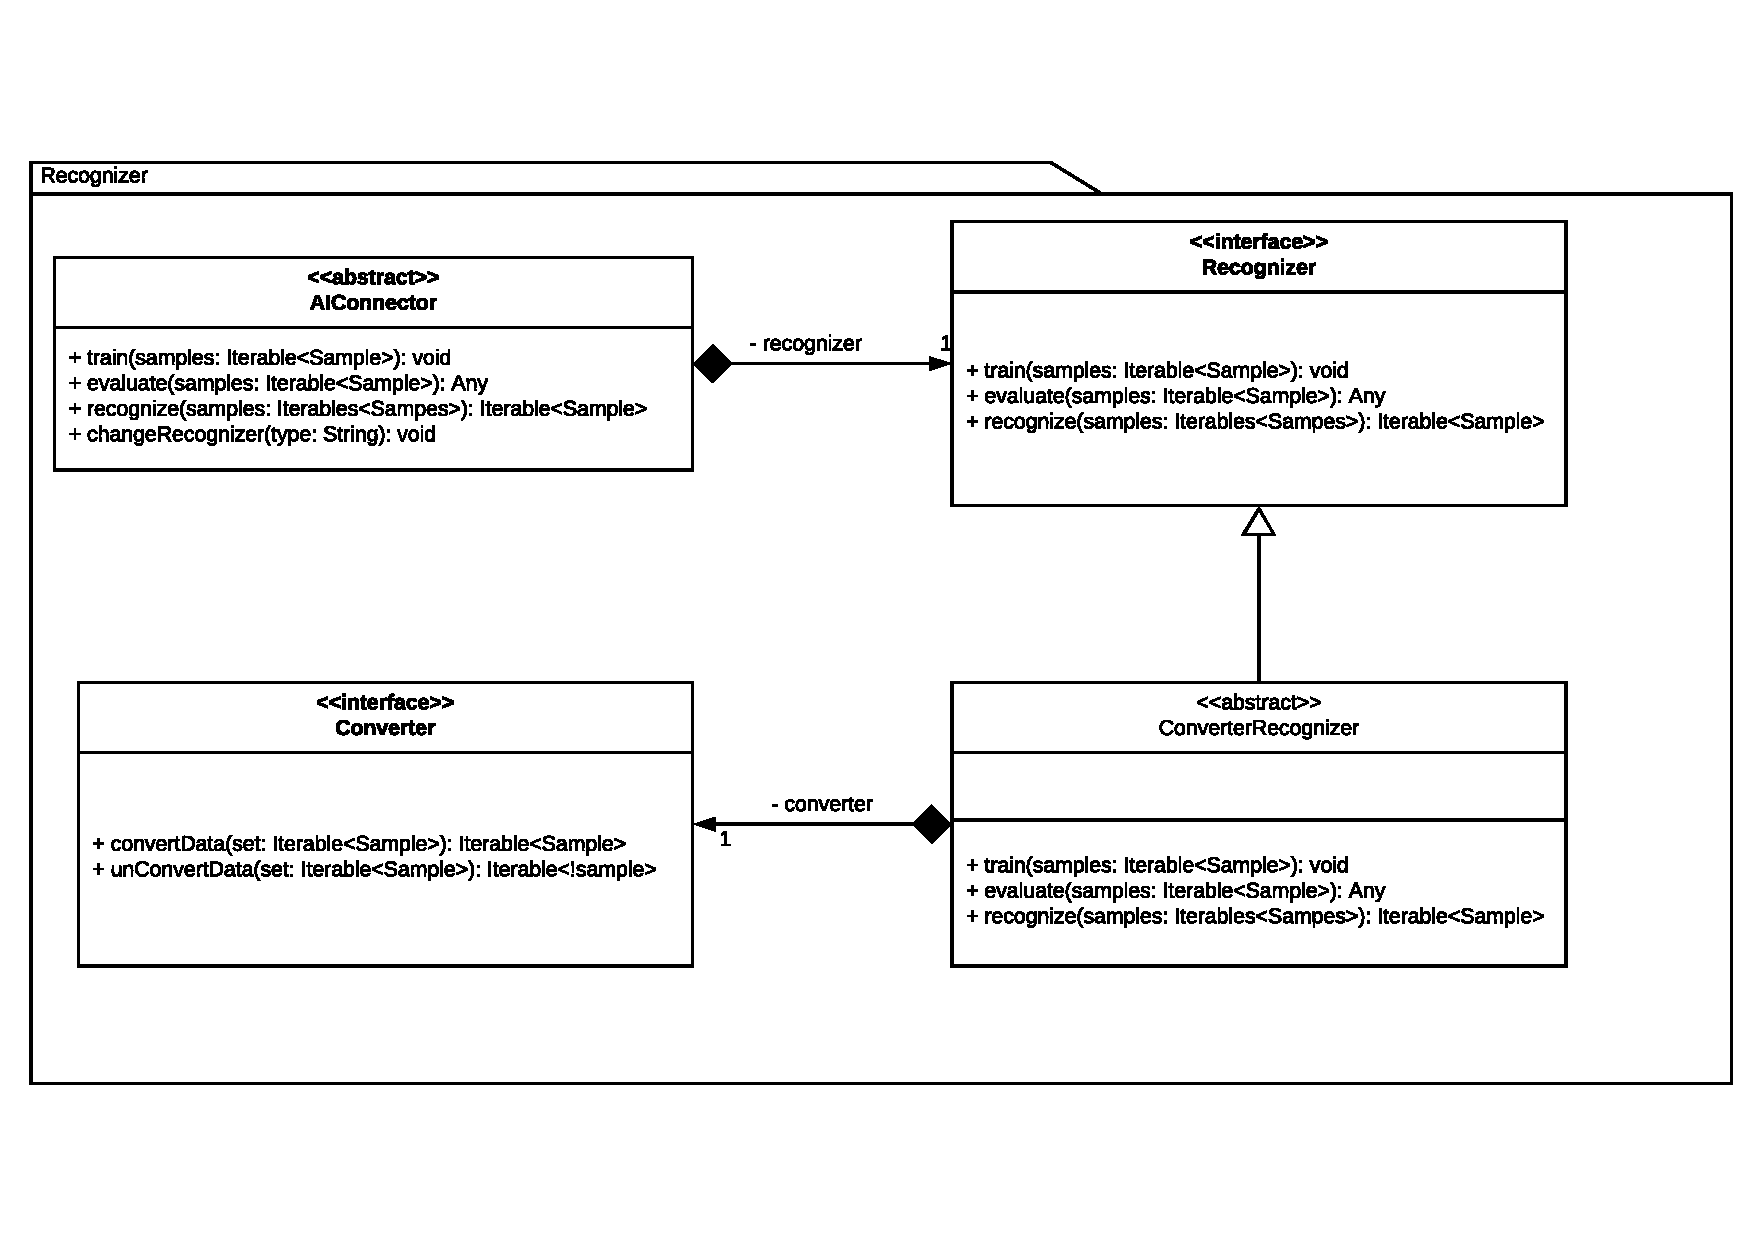
\includepdf[pages=-]{assets/UML_Recognizer}

\paragraph{Architecture}

Cette partie du projet contient comme toutes les autres un connecteur qui la lie au Connector principal. Ce connecteur possède un Recognizer afin de pouvoir effectuer les opérations classiques d'entrainement, d'évaluation de celui-ci ainsi que lui demander d'effectuer une transcription. Il permet également de changer de reconnaisseur quand l'utilisateur souhaite utiliser un autre type de reconnaisseur.
Le Reconnaiseur est représenté par une interface Recognizer qui permet trois actions possibles: entrainer le reconnaisseur à partir d'un ensemble d'apprentissage, évaluer ce même reconnaisseur sur un ensemble de validation, et enfin, lui demander de transcrire un ensemble non étiqueté.
Cette interface permet notamment à l'utilisateur, de connecter son propre reconnaisseur, et même s'il le souhaite, d'en créer un au sein de l'application. elle est également la seule qu'il est obligé d'implémenter pour faire fonctionner l'ensemble. Cependant, il faut dans certains cas convertir les données dans la base de donnée en données compréhensibles par le reconnaisseur. Ainsi, deux autres interfaces sont nécessaires: une interface Converter permettant la convertion des données entrantes et sortantes du reconnaisseur ainsi qu'une classe abstraite ConverterRecognizer héritant de Recognizer et possédant un convertisseur adapté au reconnaisseur utilisé.

%-----------------------------------------------------------------------------------------------------------------------
\section{Contrôleur}

Le rôle du contrôleur est de mettre en relation les 4 parties du projet : le \textit{frontend}, \textit{i.e.} l'interface homme-machine, la base de données, ainsi que le traitement des données. Pour ce faire, nous avons 4 classes abstraites, un connecteur par \textit{package} du projet, chacun possédant des méthodes générales, qui appellent d'autres méthodes de leurs \textit{packages} respectifs. Cela permet d'avoir un objet \texttt{Controller} central qui manipule tous les éléments du projet avec un code très lisible. Nous fournissons une implémentation de chaque connecteur, pour le bon fonctionnement du projet. Une fabrique est également prévue. En effet, le contrôleur récupèrera les instances des connecteurs à partir de cette fabrique. Cela permet à l'utilisateur de changer d'instance de connecteur en changeant une ligne de code seulement.

\chapter{Diagrammes de séquence}

% ---

\chapter{Conclusion}

Dans le cadre de notre 4\up{ème} année en informatique, nous avons pour mission de
mener à bien un projet de manière plus précise et plus structurée qu’en 3\up{ème} année.
Notre projet, en partenariat avec les archives départementales d’Ille-et-Vilaine,
l’équipe IntuiDoc et Doptim, consiste à créer un logiciel qui aidera les chercheurs et
les ingénieurs à faire progresser la reconnaissance d’écriture manuscrite, afin de rendre
des documents anciens plus accessibles et plus compréhensibles.

\paragraph{}
Notre groupe se compose de 8 étudiants : Enzo CRANCE, Kevin DESPOULAINS, Timothée NEITTHOFFER,
Laure DU MESNILDOT, Charlotte RICHARD, Valentin FOUCHER, Gaël GENDRON et Corentin GUILLOUX.
3 d’entre nous partiront en mobilité internationale au second semestre : Kevin DESPOULAINS,
Gaël GENDRON et Corentin GUILLOUX. Il nous faudra ainsi prendre en compte dans la réalisation
de notre projet ce changement d’effectif. L’étude du projet, la répartition des tâches et la
planification ont donc été faites bien en amont des phases de développement pour permettre à
ceux qui seront encore présents au second semestre de ne pas prendre de retard.

\paragraph{}
Nous avons dans un premier temps étudié ce qui nous était demandé de faire avant de
décider des technologies que nous allions utiliser. Nous avons bien sûr commencé à
étudier les différents outils (langages, API, etc.) que nous pourrions utiliser et qui
feront l’objet du prochain rapport.

\paragraph{}
Nous avons ensuite rédigé notre cahier des charges en reprenant les différentes fonctionnalités
que nous souhaitons développer, en accord avec Bertrand COÜASNON, tout en prenant en compte
les éléments extérieurs avec lesquels notre programme doit communiquer.

\paragraph{}
Nous avons également distribué les rôles qui nous semblent importants pour veiller au bon
déroulement du projet sans mettre trop de pression sur les personnes les endossant.
Un planning prévisionnel a également été rédigé.

%\newpage
%\bibliography{main}
%\bibliographystyle{plain}

\chapter{Annexes}


\includepdf[pages=-]{pagen.pdf}
\end{document}
